\chapter{Implémentation de la méthode linéaire dans Antares}

%Le plan du rapport doit être équilibré, c’est-à-dire que les paragraphes, à l’intérieur de chacune des deux parties principales (I. Présentation de l’entreprise, II. Présentation du travail réalisé) doivent être à peu près d’égale mesure. On évitera, par exemple, le mélange de paragraphes de 3 lignes avec d’autres de 60 lignes ; le rapport entre ces petits blocs de texte doit rester de 1 à 3.`

%– Le récit de l’expérience préprofessionnelle doit faire état de toutes les fonctions exercées par le stagiaire à son poste. Il doit comporter des développements techniques (illustrés par des schémas expliqués et commentés, par exemple), mais il s’agit avant tout de donner au lecteur une idée de ce que furent l’emploi du temps du stagiaire, ses tâches quotidiennes, les contraintes du métier, la nature des relations humaines dans cet environnement, les difficultés rencontrées et les résultats obtenus.
%– Les connaissances techniques acquises doivent transparaître dans le document. Le correcteur évaluera si celui-ci fait état d’une maîtrise réelle des outils (informatiques, mécaniques, etc.) utilisés pendant le stage. En outre, il estimera le niveau des connaissances techniques acquises que la rédaction du rapport aura su mettre en évidence.


Le stage a débuté au début du mois de juin 2024. Un ordinateur et un PIN-pad générateur d'\ac{OTP} ont été mis à ma disposition. Carlos, mon maître de stage, m'a fourni les informations nécessaires pour comprendre et utiliser Antares\cite{antares}, une librairie de développement, à l'aide de la documentation en ligne\footnote{Documentation d'Antares : \href{https://cerfacs.fr/antares/}{cerfacs.fr/antares}}. Ensuite j'ai résolu un bug mineur sur Antares, ce qui m'a permis de me familiariser avec Nitrox, le Gitlab hébergé sur le serveur du CERFACS où sont situés Antares et d'autres codes du CERFACS.


\section{La librairie Antares}

Antares est une librairie Python d'environ trois cents \ac{Mo}, composée de près de trois mille fichiers, incluant environ cinquante traitements. Un traitement est ce qui permet de faire une vue en coupe, de l'interpolation, etc.
Elle s'appuie fortement sur la librairie numpy afin de profiter des leurs algorithmes optimisés.
Elle permet de visualiser, traiter, réorganiser des données de simulation numérique issues de différents solveurs utilisés par le CERFACS et ses partenaires. Ces données sont organisées par Antares de manière unique et commune, ce qui est une grande force, notamment pour le partage et l'optimisation des post-traitements.

% Aussi je me rend compte que tu n'as jamais vraiment expliqué comment les traitements fonctionnent. C-a-d que ce sont des dictionnaires dans lesquels tu spécifies des mot clés / paramètres pour contrôler le comportement du traitement. Tu pourra le rajouter dans la partie de description Antares
Chaque traitement est une classe composée liste de mots-clefs qui correspondent à chaque paramètre. Certains sont donnés nécessairement à donner par l'utilisateur, d'autres sont initialisés par défaut et peuvent être modifiés ou non. Nous retrouvons les deux paramètres 'source' et 'target' nécessaires au traitement d'interpolation ligne 3 et 4 de l'exemple de code \ref{lst:antares_2}. Les autres arguments du traitement d'interpolation sont listés plus bas \ref{arguments}.


Une solution CFD est interprété par Antares comme une "Base".
Cette dernière peut être constituée d'une ou plusieurs zones.
Une zone représente un emplacement physique de la solution (par exemple, pour une chambre de combustion, nous pourrions avoir deux zones, régis avec des équations différentes: une avant les injecteurs et une après). % A vérifier par Carlos 
Chaque zone peut avoir un ou plusieurs instants.
Un instant est une "capture" de la solution à un instant t. Cela peut être la solution finale de la simulation par exemple. Plusieurs instants peuvent représenter une simulation dynamique qui est utile dans le cas de l'aéroacoustique par exemple, où nous cherchons l'évolution temporelle de la pression.
Dans le cas où la structure du maillage ne change pas entre deux instants, les positions peuvent être définies dans la zone et seule les variables changent entre les instants. On parle dans ce cas d'"instant partagé".\label{instants_partages}

% Généralement les instants sont identiques entre les zones, on dit qu'ils sont "partagés" tq les variables Carlos ?

Nous y retrouvons les variables et leurs valeurs sur le maillage de la zone et instant en question

% Ensuite chaque zone a un ou plusieurs instants où nous pouvons trouver la solution d'une variable, qui sera de même dimension que les coordonnées de l'instant.

La structure des solutions CFD interprétées dans Antares est illustrée ci-dessous (figure \ref{fig:structure_antares}):

\begin{figure}[H]
\centering
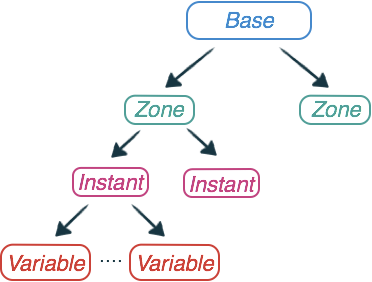
\includegraphics[width=0.42\textwidth]{images/data_structure_1.png}
\caption{Structure des données (source: \href{https://cerfacs.fr/antares/src/tutorial/base.html}{Antares Tutorial})}
\label{fig:structure_antares}
%\footnote{Source:https://cerfacs.fr/antares/src/tutorial/base.html}
%\label{fig:https://cerfacs.fr/antares/src/tutorial/base.html}
\end{figure}

Voici un exemple d'utilisation d'Antares :

\begin{lstlisting}[caption=Exemple simple d'utilisation d'Antares pour interpoler, label={lst:antares_2}]
    import antares
    myt = antares.Treatment('interpolation')
    myt['source'] = source_base
    myt['target'] = target_base
    result = myt.execute()
\end{lstlisting}

Dans le cas ci-dessus, \texttt{result[0][0]['variable1']} est un tableau numpy utilisable par l'utilisateur.

Un point important pour l'interpolation linéaire est la connectivité. Si le maillage est non structuré, alors, chaque cellule est définie par un type de forme et par ses sommets. Par exemple, elle peut être donnée par \texttt{base[0][0].connectivity['tri']} si la base contient des triangles (équivalent à avoir une connectivité "tri") dans sa zone 0 à l'instant 0.


\section{Les différentes méthodes d'interpolation}

L'interpolation consiste à déterminer la valeur de nouveaux points à partir de la valeur de points existants. En voici un exemple en \ac{1D} (l'axe x représente la position et l'axe y la valeur des points).

\vspace{0,5cm}


\begin{figure}[ht!]
    \centering
    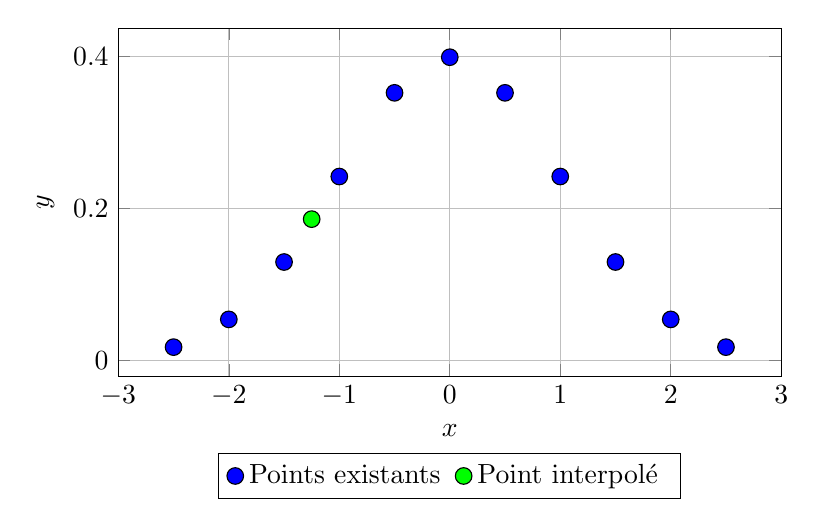
\begin{tikzpicture}
        \begin{axis}[
            width=10cm,
            height=6cm,
            xlabel={$x$},
            ylabel={$y$},
            grid=major,
            legend style={at={(0.5,-0.22)}, anchor=north, legend columns=-1},
        ]
    
        % Points existants (bleus) sur la courbe en cloche
        \addplot[
            only marks,
            mark=*,
            mark options={scale=1.5, fill=blue},
        ] coordinates {
            (-2.5, 0.0175)
            (-2, 0.05399)
            (-1.5, 0.1295)
            (-1, 0.24197)
            (-0.5, 0.35207)
            (0, 0.39894)
            (0.5, 0.35207)
            (1, 0.24197)
            (1.5, 0.1295)
            (2, 0.05399)
            (2.5, 0.0175)
        };        
        \addlegendentry{Points existants \hspace{0,3cm}}
    
        % Point interpolé (vert)
        \addplot[
            only marks,
            mark=*,
            mark options={scale=1.5, fill=green},
        ] coordinates {
            (-1.25, 0.1859)
            };
        \addlegendentry{Point interpolé \hspace{0,3cm}}
    
        \end{axis}
    \end{tikzpicture}
    \caption{Schéma d'interpolation avec des points sur une courbe en cloche}
    \label{fig:interpolation_cloche_points}
\end{figure}

    
\vspace{0,5cm}

Dans ce paragraphe, nous allons présenter les types d'interpolation\cite{cassiopee2015} implémentables dans Antares.

Cela implique certaines conditions, notamment sur le type de maillage.

Un maillage structuré est un maillage dont la connectivité entre les points peut être décrite de manière régulière, généralement à l'aide de tableaux multidimensionnels (1D, 2D, 3D). Dans un tel maillage, les points sont organisés en une grille régulière, ce qui permet de naviguer facilement à travers les données sans avoir à spécifier explicitement les relations entre les points.

En revanche, un maillage non structuré est un maillage où les éléments (cellules) sont définis par des formes géométriques quelconques et où la connectivité des points ne suit pas un schéma régulier. Cela signifie que chaque cellule doit spécifier explicitement les points qui la composent. Ces maillages sont souvent utilisés pour modéliser des géométries complexes où une grille régulière serait inadaptée.

Dans Antares, nous visons à traiter des maillages non structurés, car ils sont couramment utilisés dans les simulations modernes en raison de leur flexibilité à représenter des géométries complexes.

Un facteur à prendre en compte dans la méthode que l'on souhaite implémenter est aussi le temps de calcul, appelé 'coût'.

La caractérisation mathématique des équations à interpoler est probablement le paramètre le plus important à prendre en compte, mais aussi assurément le plus difficile. Les équations dont sont issues les solutions numériques en entrée dans Antares sont très difficiles à caractériser mathématiquement (tel que l'équation de Naviers-Stokes) et le niveau en mathématiques est trop élevé pour pouvoir se plonger en profondeur sur ce problème\cite{gordont1971_2}. C'est pour cela qu'il n'y aura pas beaucoup de résultats mathématiques à présenter dans cette partie.
Heureusement, ces méthodes ont déjà été implémentées et testées pour d'autres codes de simulation numérique, ce qui permet de nous donner une bonne idée des résultats que nous pouvons espérer.


hip est un logiciel créé en 1997 au CERFACS pour convertir des maillages multiblocs structurés en maillages non structurés.
Différentes méthodes d'interpolation y sont codés et décrites dans le guide utilisateur\cite{muller2020}. Cette référence pourrait être lue avant d'implémenter une potentielle future interpolation dans Antares.

%\addcontentsline{toc}{section}{L'interpolation et l'aéroacoustique}

\subsection{La méthode par voisin le plus proche}
Cette première méthode est très simple : nous prenons comme valeur \( v \) d'interpolation au point \( p \) la valeur \( v \) du point le plus proche de \( p \).
En voici quelques illustrations :

%\vspace{0.5cm}

\begin{figure}[ht!]
    \centering
        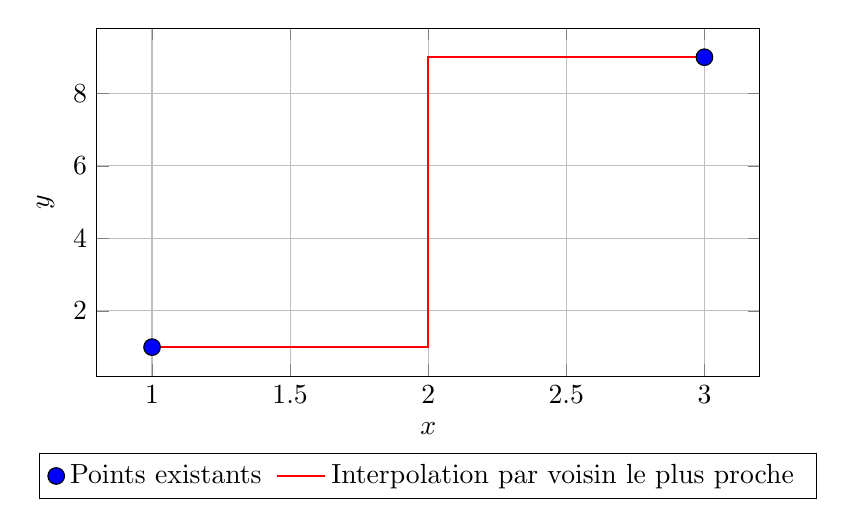
\begin{tikzpicture}
            \begin{axis}[
                width=10cm,
                height=6cm,
                xlabel={$x$},
                ylabel={$y$},
                grid=major,
                legend style={at={(0.5,-0.22)}, anchor=north, legend columns=-1},
            ]

            \addplot[
                only marks,
                mark=*,
                mark options={scale=1.5, fill=blue},
            ] coordinates {
                (1, 1)
                (3, 9)
            };
            \addlegendentry{Points existants \hspace{0,3cm}}

            \addplot[
                thick,
                red,
            ] coordinates {
                (1, 1)
                (2, 1)
                (2, 9)
                (3, 9)
            };
            \addlegendentry{Interpolation par voisin le plus proche \hspace{0,3cm}}

            %\addplot[
            %    only marks,
            %    mark=*,
            %    mark options={scale=1.5, fill=green},
            %] coordinates {
            %    (1.7, 1)
            %};
            %\addlegendentry{Point interpolé}

            \end{axis}
        \end{tikzpicture}
    \caption{Schéma d'interpolation par voisin le plus proche}
    \label{fig:interpolation_voisin}
\end{figure}

La courbe La courbe rouge représente l'interpolation sur tout le domaine x entre les deux points. Cela représente les coordonnées (x, y) de tous les potentiels points d'interpolation.

Cette méthode est discontinue et peu précise pour la plupart des fonctions.



\subsection{La méthode pondération inverse à la distance (IDW)} % déjà '\ac'

Probablement l'interpolation la plus simple après la méthode du voisin le plus proche (toujours dans notre cas d'application), cette méthode est la seule qui était implémentée dans Antares (elle inclut aussi la méthode du voisin le plus proche comme expliqué plus tard dans cette section). Elle a pour formule :

\[
\hat{f}(x) = \frac{\sum_{i=1}^{N} \frac{f(x_i)}{d(x, x_i)^p}}{\sum_{i=1}^{N} \frac{1}{d(x, x_i)^p}}
\]

où :

- \(\hat{f}(x)\) est la valeur interpolée à la position \(x\),

- \(f(x_i)\) est la valeur connue aux points de données \(x_i\),

- \(d(x, x_i)\) est la distance entre \(x\) et \(x_i\),

- \(p\) est le paramètre de puissance,

- \(N\) est le nombre total de points de données.

\vspace*{0,5cm}

Pour éviter une division par 0, très proche d'un point existant, le point interpolé prendra la valeur du point existant. Cette distance est définie à 1e-10 dans le traitement et peut être modifiée par l'utilisateur en ajustant l'argument \texttt{'tolerance'} en ajoutant la ligne :
\begin{lstlisting}[]
    myt['tolerance'] = valeur
\end{lstlisting}
entre la ligne 2 et 5 de l'exemple présenté dans la partie '2.1 La librairie Antares'.
Il en est de même pour les paramètres \(N\) et \(p\) avec pour argument respectivement \texttt{'nb\_points'} et \texttt{'invdist\_power'}.


\vspace*{0,5cm}


En voici des illustrations 1D :

\begin{figure}[ht!]
    \centering
    \begin{minipage}{0.45\textwidth}
        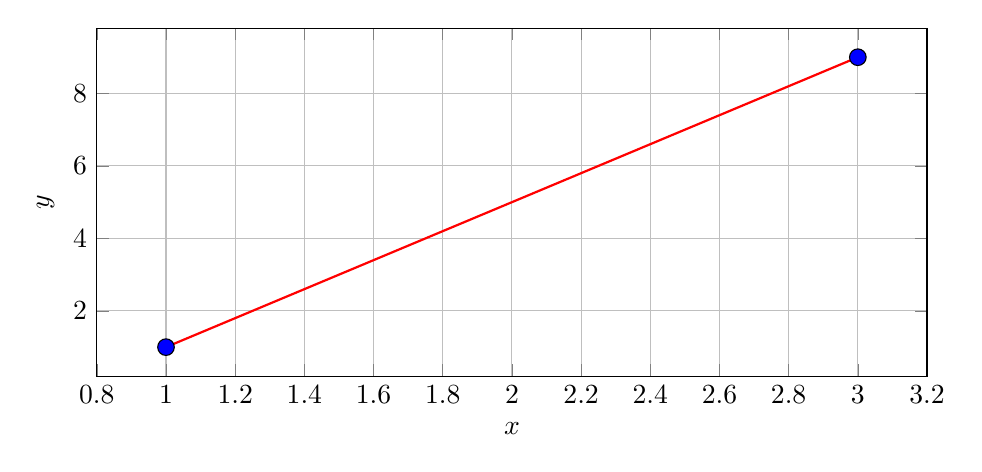
\begin{tikzpicture}
            \begin{axis}[
                width=\textwidth,
                height=6cm,
                xlabel={$x$},
                ylabel={$y$},
                grid=major,
            ]
            \addplot[
                only marks,
                mark=*,
                mark options={scale=1.5, fill=blue},
            ] coordinates {
                (1, 1)
                (3, 9)
            };

            \addplot[
                domain=1:3,
                samples=100,
                smooth,
                thick,
                red,
            ] {(1/abs(1-x) + 9/abs(x-3))/(1/(abs(1-x))+1/(abs(x-3)))};

            %\addplot[
            %    only marks,
            %    mark=*,
            %    mark options={scale=1.5, fill=green},
            %] coordinates {
            %    (2, 5)
            %};
            \end{axis}
        \end{tikzpicture}
        \caption{Interpolation IDW N=2, p=1}
    \end{minipage}
    \hspace{0.5cm}
    \begin{minipage}{0.45\textwidth}
        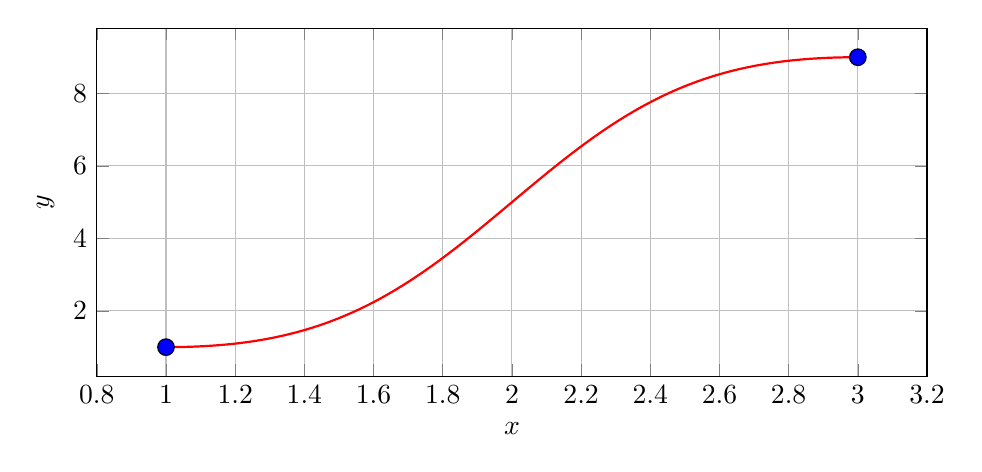
\begin{tikzpicture}
            \begin{axis}[
                width=\textwidth,
                height=6cm,
                xlabel={$x$},
                ylabel={$y$},
                grid=major,
            ]
            \addplot[
                only marks,
                mark=*,
                mark options={scale=1.5, fill=blue},
            ] coordinates {
                (1, 1)
                (3, 9)
            };

            \addplot[
                domain=1:3,
                samples=100,
                smooth,
                thick,
                red,
            ] {(1/(abs(1-x)^2) + 9/(abs(x-3)^2))/(1/(abs(1-x)^2)+1/(abs(x-3)^2))};

            %\addplot[
            %    only marks,
            %    mark=*,
            %    mark options={scale=1.5, fill=green},
            %] coordinates {
            %    (2, 5)
            %};
            \end{axis}
        \end{tikzpicture}
        \caption{Interpolation IDW N=2, p=2}
    \end{minipage}

    \vspace{0.5cm}

    \begin{minipage}{0.45\textwidth}
        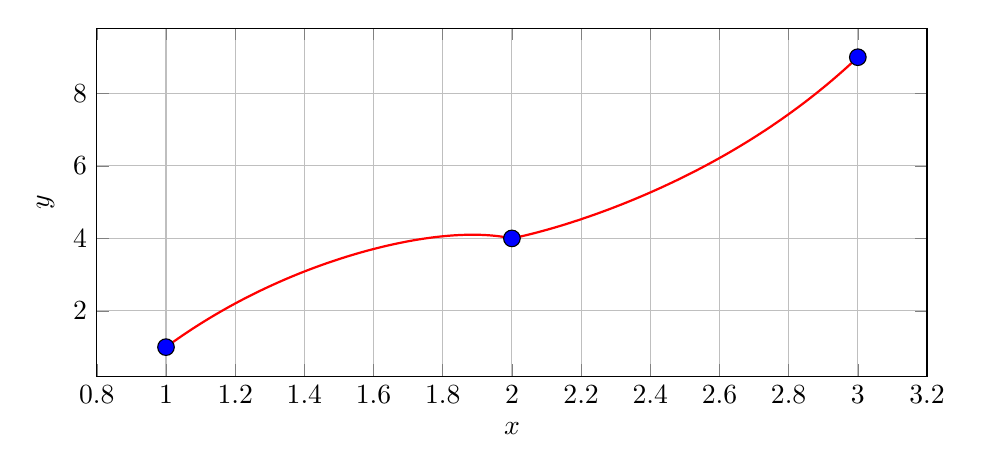
\begin{tikzpicture}
            \begin{axis}[
                width=\textwidth,
                height=6cm,
                xlabel={$x$},
                ylabel={$y$},
                grid=major,
            ]
            \addplot[
                only marks,
                mark=*,
                mark options={scale=1.5, fill=blue},
            ] coordinates {
                (1, 1)
                (3, 9)
                (2, 4)
            };

            \addplot[
                domain=1:3,
                samples=100,
                smooth,
                thick,
                red,
            ] {(1/abs(1-x) + 9/abs(x-3) + 4/abs(2-x))/(1/(abs(1-x)) + 1/(abs(x-3)) + 1/(abs(2-x)))};

            %\addplot[
            %    only marks,
            %    mark=*,
            %    mark options={scale=1.5, fill=green},
            %] coordinates {
            %    (1.5, 3.43)
            %};
            \end{axis}
        \end{tikzpicture}
        \caption{Interpolation IDW N=3, p=1}
    \end{minipage}
    \hspace{0.5cm}
    \begin{minipage}{0.45\textwidth}
        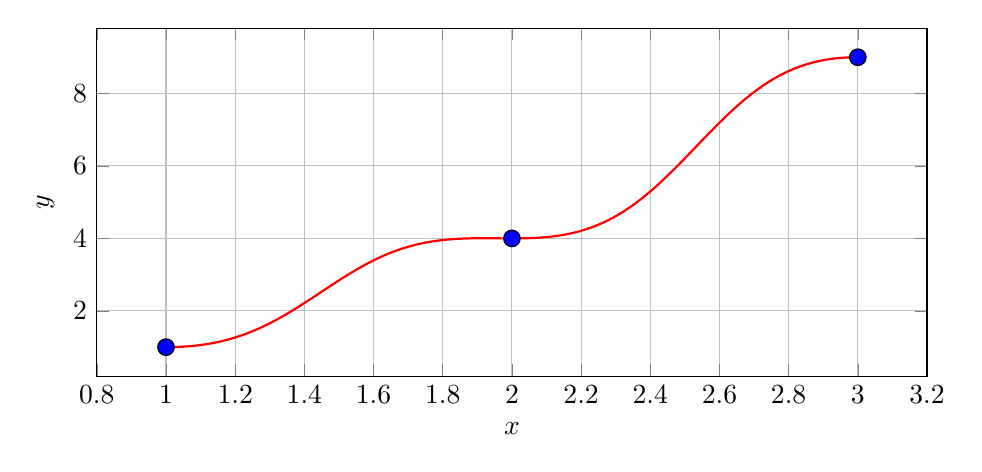
\begin{tikzpicture}
            \begin{axis}[
                width=\textwidth,
                height=6cm,
                xlabel={$x$},
                ylabel={$y$},
                grid=major,
            ]
            \addplot[
                only marks,
                mark=*,
                mark options={scale=1.5, fill=blue},
            ] coordinates {
                (1, 1)
                (3, 9)
                (2, 4)
            };

            \addplot[
                domain=1:3,
                samples=100,
                smooth,
                thick,
                red,
            ] {(1/(abs(1-x)^2) + 9/(abs(x-3)^2) + 4/(abs(2-x)^2))/(1/(abs(1-x)^2) + 1/(abs(x-3)^2) + 1/(abs(2-x)^2))};

            %\addplot[
            %    only marks,
            %    mark=*,
            %    mark options={scale=1.5, fill=green},
            %] coordinates {
            %    (1.5, 2.84)
            %};
            \end{axis}
        \end{tikzpicture}
        \caption{Interpolation IDW N=3, p=2}
    \end{minipage}
\end{figure}

\vspace{-0.5cm}

\begin{figure}[H]
    \centering
    
\includegraphics[width=0.39\textwidth]{images/legende-interp3.png}
\end{figure}


Dans notre cas, nous ne prenons pas en compte tous les points du maillage source. Nous nous limitons à un nombre \(N\) de points les plus proches. Cela implique une discontinuité lorsque nous changeons de point. Pour illustrer cela, voici une figure 1D où tous les points sont espacés d'une unité. Avec \(N\)=3, cela revient ici à changer l'un des trois points de calcul pour une valeur de \(x\) égale à 0,5 modulo un. Le modulo un est représenté par une ligne en pointillés noirs. Il est appelé rayon, car en 2D, il est représenté par un cercle et en 3D pas une sphère. 

\begin{figure}[ht!]
\centering
    \begin{tikzpicture}
        \begin{axis}[
            width=10cm,
            height=6cm,
            title={Interpolation IDW (N=3, p=2, rayon=1)},
            xlabel={$x$},
            ylabel={$y$},
            grid=major,
            legend style={at={(0.5,-0.22)}, anchor=north, legend columns=-1},
        ]
        \addplot[
            only marks,
            mark=*,
            mark options={scale=1.5, fill=blue},
        ] coordinates {
            (1, 1)
            (2, 4)
            (3, 9)
        };
        \addlegendentry{Points existants\phantom{---}}
    
        % Plotting the radius for the nearest neighbors
        \addplot[dashed, aurometalsaurus, thick] coordinates {(1.5, 0) (1.5, 9)};
        \addlegendentry{Rayon de 1\phantom{---}}
    
        \addplot[
            domain=1:1.5,
            samples=100,
            smooth,
            thick,
            red,
        ] {(1/(abs(1-x)^2) + 4/(abs(x-2)^2))/(1/(abs(1-x)^2)+1/(abs(x-2)^2))};
        \addplot[
            domain=1.5:2.5,
            samples=100,
            smooth,
            thick,
            red,
        ] {(1/(abs(1-x)^2) + 9/(abs(x-3)^2) + 4/(abs(2-x)^2))/(1/(abs(1-x)^2) + 1/(abs(x-3)^2) + 1/(abs(2-x)^2))};
        \addplot[
            domain=2.5:3,
            samples=100,
            smooth,
            thick,
            red,
        ] {(4/(abs(x-2)^2) + 9/(abs(3-x)^2))/(1/(abs(x-2)^2)+1/(abs(3-x)^2))};
        \addlegendentry{Interpolation IDW}
    
        \addplot[dashed, aurometalsaurus, thick] coordinates {(2.5, 0) (2.5, 9)};
    
        \end{axis}
    \end{tikzpicture}
    \caption{Schéma d'interpolation IDW avec rayon}
    %\label{fig:interpolation_IDW_rayon}
\end{figure}

Nous observons une discontinuité en 1,5 et 2,5. La discontinuité peut être un grand problème pour la stabilité des schémas numériques.

\begin{comment}
    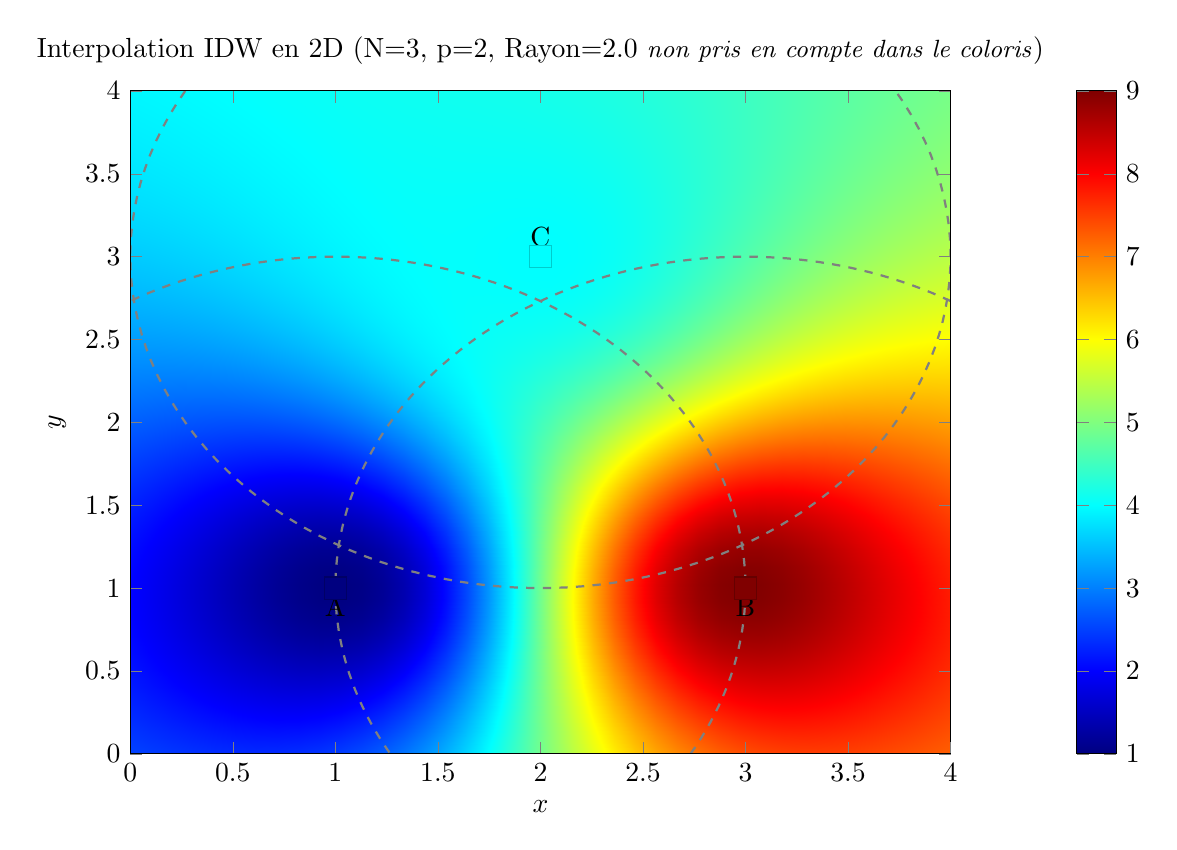
\begin{tikzpicture}
        \begin{axis}[
            view={0}{90},
            xlabel={$x$},
            ylabel={$y$},
            colorbar,
            title={Interpolation IDW en 2D (N=3, p=2, Rayon=2.0 {\small \textit{non pris en compte dans le coloris}})},
            colormap/jet,  % Utilisation d'une colormap standard
            width=12cm,
            height=10cm,
        ]

        % Points d'interpolation connus
        \pgfplotstableread{
            x y z
            1 1 1
            3 1 9
            2 3 4
        }\datatable

        % Fonction IDW
        \addplot3[
            surf,
            shader=interp,
            domain=0:4,
            y domain=0:4,
            samples=40,    % A augementer avant la version finale
        ] 
        {(1/(sqrt((x-1)^2+(y-1)^2 + 1e-6)^2) + 
        9/(sqrt((x-3)^2+(y-1)^2 + 1e-6)^2) + 
        4/(sqrt((x-2)^2+(y-3)^2 + 1e-6)^2)) / 
        (1/(sqrt((x-1)^2+(y-1)^2 + 1e-6)^2) + 
        1/(sqrt((x-3)^2+(y-1)^2 + 1e-6)^2) + 
        1/(sqrt((x-2)^2+(y-3)^2 + 1e-6)^2))};
        
        % Points d'interpolation connus
        \addplot3[
            only marks,
            scatter,
            scatter src=explicit,
            point meta=\thisrow{z},
            mark=square*,
            mark options={scale=2},
        ] table [x=x, y=y, z=z] {\datatable};

        % Tracer les cercles de rayon 2
        \addplot[
            draw=gray, 
            thick, 
            dashed, 
            domain=-30:120,
            samples=100,
        ] 
        ({1 + 2*cos(x)}, {1 + 2*sin(x)});  % Cercle autour du point A (1,1)

        \addplot[
            draw=gray, 
            thick, 
            dashed, 
            domain=60:210,
            samples=100,
        ] 
        ({3 + 2*cos(x)}, {1 + 2*sin(x)});  % Cercle autour du point B (3,1)

        \addplot[
            draw=gray, 
            thick, 
            dashed, 
            domain=-210:30,
            samples=100,
        ] 
        ({2 + 2*cos(x)}, {3 + 2*sin(x)});  % Cercle autour du point C (2,3)

        % Annoter les points
        \node at (axis cs:1,1,1) [anchor=north] {A};
        \node at (axis cs:3,1,9) [anchor=north] {B};
        \node at (axis cs:2,3,4) [anchor=south] {C};

        \end{axis}
    \end{tikzpicture}
\end{comment}

Nous pouvons aussi imaginer que 2 points, A et B, à droite et à gauche d'une ligne verticale de 3 points (les plus proches), prendront la même valeur pour \( N \) = 3 :

\begin{figure}[ht!]
    \centering
    \begin{tikzpicture}

        % Les points sur la ligne verticale
        \filldraw[blue] (0, -1.2) circle (2pt) node[right] {$c$}; 
        \filldraw[blue] (0, 0) circle (2pt) node[right] {$b$};
        \filldraw[blue] (0, 1.5) circle (2pt) node[right] {$a$};
        
        % Les autres
        \filldraw[blue] (-4, -0.5) circle (2pt) node[above left] {$d$};
        \filldraw[blue] (5, 1.0) circle (2pt) node[above right] {$e$};
    
        % Les points à gauche et à droite qui prennent la même valeur
        \filldraw[red] (-1.5, 0.5) circle (2pt) node[above left] {A}; 
        \filldraw[red] (1.5, 0.5) circle (2pt) node[above right] {B};
    
        % Lignes de liaison entre les points rouges et les trois plus proches voisins
        \draw[dashed, gray] (-1.5, 0.5) -- (0, -1.2);
        \draw[dashed, gray] (-1.5, 0.5) -- (0, 0);
        \draw[dashed, gray] (-1.5, 0.5) -- (0, 1.5);
    
        \draw[dashed, gray] (1.5, 0.5) -- (0, -1.2);
        \draw[dashed, gray] (1.5, 0.5) -- (0, 0);
        \draw[dashed, gray] (1.5, 0.5) -- (0, 1.5);
    
    \end{tikzpicture}
    
    \caption{Schéma montrant la non-directivité d'IDW}
    %\label{fig:interpolation_IDW_rayon}
\end{figure}

    
Ce qui n'est pas cohérent dans le cas où le gradient selon l'horizontal n'est pas nul.

\begin{comment}
Un des problèmes avec la méthode IDW est que « \textit{a directional bias to the database solutions can shift the interpolated results} »\footnote{Traduction : « un biais directionnel dans les solutions de la base de données peut décaler les résultats interpolés. » Source : \textit{Titre de l'article}, Auteur, Année, URL si applicable.}.
\end{comment}


Un des problèmes avec la méthode IDW est que « un biais directionnel dans les solutions de la base de données peut décaler les résultats interpolés »\cite{palmer2009}. % \footnote{Traduction de : « \textit{One issue with the IDW method is that a directional bias to the database solutions can shift the interpolated results.} »


Lorsque toutes les informations selon un axe de l'espace ne se situent que d'un côté, le gradient ne sera pas pris en compte et l'erreur sera élevée. Par exemple, cela est généralement le cas lorsque le maillage cible a des points qui ne sont pas compris dans le maillage source.

D'autres méthodes dérivées ou similaires existent pour évaluer nos poids (les poids sont les distances inverses à la puissance p dans notre cas). La plus intéressante serait celle dite de Franke-Littke. Elle consiste à utiliser une distance maximale autour du point au-delà de laquelle les autres points ne sont pas pris en compte. Autrement dit, on utilise un cercle (dans le cas 2D) d'un certain rayon pour déterminer quels points nous sont utiles pour l'interpolation. Dans ce cas le nombre de points est variable.
J'ai considéré subjectivement que cette méthode n'était pas intéressante. La méthode confrontée à un maillage ayant une différence de raffinement intrinsèque importante, ne prendrais aucun point à certains endroits et dans d'autres lieux, un trop grand nombre de points devrait être calculé.

\begin{comment}
    Certaines conditions de cette méthode doivent être respectés, comme Pour N tends vers l’infini, p doit être inférieur ou égale à la dimension, par ex 3 pour ne pas diverger. Mais N n’est pas grand dans notre cas.
    Voir d'autres choses page 7 de mon ppt.
\end{comment}


Par défaut, dans le code, \(p\) est égal à '1' et \(N\) est égale aux nombre de sommets de la première cellule de la liste de types de cellules de la base cible. Il y aurait peut-être une modification mineure à faire sur ce point. La structure de la base cible importe peu comparée à celle de la base source, pour l'interpolation. Mais par soucis de rétrocompatibilité, aucune modification ne doit changer l'utilisation qui a déjà été faite de ce traitement. % ! test à faire ici !

Nous remarquons que pour \( N = 1 \), nous retrouvons la méthode du voisin le plus proche, pour tout \( p \).
Et pour \( N = 2 \) et \( p = 1 \), toujours en 1D, nous retrouvons la méthode linéaire.

Une de mes missions était de chercher s'il y avait des paramètres plus optimisés que \(N\) et \(p\) pour cette méthode. Je n'ai pas trouvé la réponse dans les différents articles\cite{idw-arcgis} et thèses que j'ai lus. C'est pour cela que je présenterai plus tard comment j'ai trouvé des paramètres optimaux en faisant des tests.

Une des limitation\cite{idw-mapscaping} de la méthode IDW est qu'elle n'a pas d'autocorrélation spacial, contrairement à la méthode kriging que je décrirais plus tard.

\vspace{0,5 cm}




\subsection{La méthode polynomiale}

L'interpolation polynomiale est d'un degré correspondant à celui du polynôme utilisé. Elle peut être réalisée en N dimensions sur un maillage structuré. Cette interpolation est de classe \(C^\infty\) (c'est-à-dire infiniment dérivable, avec des dérivées de tous ordres continues)

\paragraph{Lagrange}
\vspace{0.5cm}
\dots
\paragraph{Hermite}
\cite{bajaj}
\vspace{0.5cm}
\dots
\paragraph{Splines}
Splines cubiques : "Notre expérience montre que les fonctions cubiques d'assemblage par spline sont très avantageuses lorsque plusieurs lignes de coordonnées intérieures généralisées sont spécifiées a priori."\cite{gordont1971}
\vspace{0.5cm}
\dots
\paragraph{NURBS}
\vspace{0.5cm}
\ac{NURBS}
Cette méthode\cite{piegl1995nurbs} pourrait être un bon candidat pour l'interpolation (sous-section de polynôme/splines ?)
\vspace{0.5cm}

\paragraph{Cubic Interpolation}
\cite{tanaka}
\vspace{0.5cm}


\subsection{Les méthodes à base de distance}
\paragraph{IDW}
\vspace{0.5cm}
Comme décrit plus tôt dans la partie 2.2.2, la méthode IDW se base sur la distance des points pour le calcul de l'interpolation.
\paragraph{Shépard}
\vspace{0.5cm}
\dots
\paragraph{RBF}
\ac{RBF}
\vspace{0.5cm}
\dots
\paragraph{DSM}
\ac{DSM}
\cite{kim2019}
\vspace{0.5cm}
\dots


%\subsection{L'interpolation par Splines}

\subsection{Méthodes géostatiques}

MLS : \cite{levin}

https://desktop.arcgis.com/fr/arcmap/latest/extensions/geostatistical-analyst/what-is-arcgis-geostatistical-analyst-.htm

Cokriging is the multivariate extension of kriging formalism, which allows to deal simultaneously with two or more variables defined over the same domain and to account for additional information about spatial correlation between the variables :
https://www.sciencedirect.com/topics/agricultural-and-biological-sciences/kriging


"We specifically use the Gaussian RBF and the Exponential Dot Product Kernels to do the interpolations, and approximate the benchmark called Franke's Function." : https://bitbucket.org/joelrosenfeld/rbf-and-kernel-interpolation/src/master/

"The Moving Least Squares (MLS) method is a meshless numerical technique used for solving partial differential equations (PDEs) and reconstructing functions from scattered data, especially in cases where the data points are irregularly spaced or unstructured.
Ligne a decomenter%" : https://www.sciencedirect.com/topics/mathematics/moving-least-squares#:~:text=The%20Moving%20Least%20Squares%20(MLS,are%20irregularly%20spaced%20or%20unstructured.


Expliquer voronoï

Pour prochaine méthode :
https://github.com/Ferrite-FEM/Ferrite.jl/blob/master/src/interpolations.jl


Super site pour ordre supérieur : https://getfem.readthedocs.io/en/latest/userdoc/appendixA.html

\subsection{Les méthode par moindres carrés}

"Piece-wise linear and minimumnorm interpolation approaches are faster than the linear least squares."\cite{muller2020}

\paragraph{Approximation des moindres carrés}
\vspace{0.5cm}
\dots
\paragraph{Moindres carrés mobiles}
\vspace{0.5cm}
\dots


\subsection{MISCOG}

Plusieurs méthodes d'interpolation d'ordre élevé sont déjà implémentées dans d'autres codes du CERFACS\cite{laborderie2018}

\subsection{La méthode linéaire}
"The linear method is simple, robust, and an acceptable choice of interpolation for rough first estimates or if the database solution variables depend linearly on design space variables. The IDW method shows no advantages over the simpler linear method and is not recommended for interpolating CFD solutions. The Kriging method gives the most accurate interpolated results and has the ability to capture non-linear behavior in the database solution variables."\cite{palmer2009}.
La littérature\cite{fluidssengineer} s'accorde à dire que l'interpolation linéaire, est la plus basique après plus proche voisin et IDW. J'entends par basique simple à implémenter, demandant peu de ressource, robuste et moyennement précise pour de l'ordre élevé. C'est pour cela que le CERFACS voulait l'implémenter dans Antares. C'est aussi la plus utilisée par Airbus, Safran et d'autres industriels (via d'autres codes qu'Antares). Cela est donc aussi intéressant d'avoir une interpolation linéaire directement dans Antares.

% Remplacer target par cible et point interpolé par cible.

\paragraph{1D}
\subparagraph{Linéaire}

En 1D, l'interpolation linéaire est simple : c'est la moyenne pondérée linéairement par la distance, des valeurs des deux points les plus proches.
Supposons que nous voulons interpoler une valeur d'un point \( p \) entre deux points \( a \) et \( b \) dans un espace 1D
et que nous représentons leurs valeurs dans une deuxième dimension \( y \).
Nous aurons alors pour formule :

\[
y_p = \frac{x_b - x_p}{x_b - x_a} \cdot y_a + \frac{x_p - x_a}{x_b - x_a} \cdot y_b
\]

%\vspace*{0.1\baselineskip}\linebreak
où \( y_p \) représente la valeur interpolée à la position \( x_p \), et \((x_a, y_a)\) et \((x_b, y_b)\) sont les points de référence. J'ai écrit cette formule afin qu'elle soit symétrique par rapport aux points \( a \) et \( b \), pour qu'ils jouent le même rôle. Ainsi elle s'entendra plus intuitivement dans des dimensions supérieures.
\vspace{0.5cm}
%\vspace*{0.1\baselineskip}\linebreak

        \( \frac{x_b - x_p}{x_b - x_a} \) est le poids pour \( y_a \) basé sur la distance relative de \( x_p \) à \( x_b \).

        \( \frac{x_p - x_a}{x_b - x_a} \) est le poids pour \( y_b \) basé sur la distance relative de \( x_p \) à \( x_a \).\vspace{0.5cm}

Ces deux termes sont pondérés de manière à ce que leur somme soit toujours égale à 1, ce
qui garantit que l'interpolation est correcte et symétrique par rapport à \( a \) et \( b \).\vspace{0.5cm}


\paragraph{2D}

\vspace{0.5cm}

En 2D, nous devons nous baser sur des surfaces, extraites de formes pour pouvoir effectuer cette pondération. En CFD, ces formes sont appelées cellules et leurs sommets nœuds. Dans notre cas, nous considérons que les variables du maillage sont contenues au niveau des nœuds. 
Il existe 3 principaux types de cellules (formes) en 2D : les triangles, les rectangles des maillages structurés (dans ce cas, la méthode est dite bilinéaire) et les quadrilatères (non croisés).
Certains industriels utilisent de plus en plus des polygones à N arrêtes. Mais pas soucis de simplicité, nous l'interpolation linéaire est limité aux 3 principales formes, les polygones pouvant être décomposés en triangles.

\subparagraph{Triangle : Barycentrique}

Pour le triangle, la méthode pour trouver la valeur au point à interpoler \( p \) est celle dite du barycentre (barycentrique).
Elle est bien documentée.

Visuellement, il faut faire la somme des valeurs aux points pondérés par la surface opposée et pondérer le tout par la surface du triangle.

\begin{comment}
    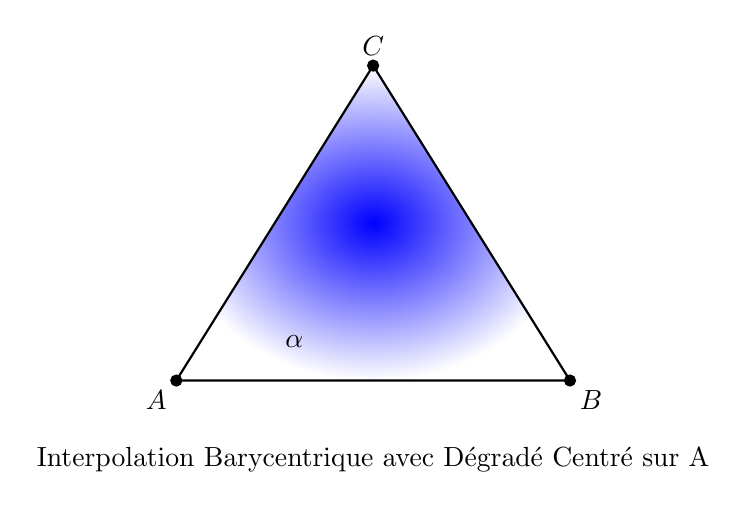
\begin{tikzpicture}
    % Triangle coordinates
    \coordinate (A) at (0,0);
    \coordinate (B) at (5,0);
    \coordinate (C) at (2.5,4);

    % Gradient fill centered at vertex A
    \shade[shading=radial, inner color=blue, outer color=white] (A) -- (B) -- (C) -- cycle;

    % Draw triangle
    \draw[thick] (A) -- (B) -- (C) -- cycle;

    % Draw labels and points
    \filldraw[black] (A) circle (2pt) node[anchor=north east] {$A$};
    \filldraw[black] (B) circle (2pt) node[anchor=north west] {$B$};
    \filldraw[black] (C) circle (2pt) node[anchor=south] {$C$};
    \node at (1.5,0.5) {$\alpha$};

    % Title
    \node at (2.5,-1) {Interpolation Barycentrique avec Dégradé Centré sur A};

\end{tikzpicture}
\end{comment}

\begin{figure}[ht!]
    \centering
    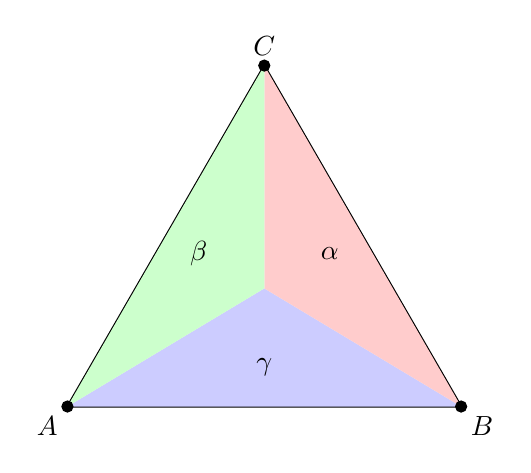
\begin{tikzpicture}

        % Define the triangle vertices
        \coordinate (A) at (0,0);
        \coordinate (B) at (5,0);
        \coordinate (C) at (2.5,4.33);
        \coordinate (P) at (2.5,1.5); % Point d'interpolation
    
        % Draw triangle
        \draw[thick] (A) -- (B) -- (C) -- cycle;
    
        % Draw Voronoi-like regions
        \fill[blue!20]  (A) -- (B) -- (P) -- cycle;
        \fill[red!20]   (B) -- (C) -- (P) -- cycle;
        \fill[green!20] (C) -- (A) -- (P) -- cycle;
        %\fill[green!20] (C) -- (barycentric cs:A=1,B=0,C=1) -- (barycentric cs:A=0,B=1,C=1) -- cycle;
    
        % Draw points
        \filldraw[black] (A) circle (2pt) node[anchor=north east] {$A$};
        \filldraw[black] (B) circle (2pt) node[anchor=north west] {$B$};
        \filldraw[black] (C) circle (2pt) node[anchor=south] {$C$};
    
        % Add labels
        \node at (barycentric cs:B=1,C=1,P=1) {$\alpha$};
        \node at (barycentric cs:C=1,A=1,P=1) {$\beta$};
        \node at (barycentric cs:A=1,B=1,P=1) {$\gamma$};
    
        % Title
        %\node at (2.5,-1) {Interpolation Barycentrique}; %Diagramme de Voronoi Modifié pour l'
    
    \end{tikzpicture}
    \label{fig:interpolation_barycentrique}
    \caption{Schéma d'interpolation barycentrique}
    %\label{fig:interpolation_IDW_rayon}
\end{figure}



Le calcul est
\begin{equation}
    \frac{\alpha y_A + \beta y_B + \gamma y_C}{\alpha + \beta + \gamma}
\end{equation}


\vspace{0.2cm}

Bien sûr, les triangles sont quelconques, mais la formule reste la même.

% Trilinéaire dans le cas où le maillage est 3D et structuré.
\subparagraph{Rectangle : bilinéaire}

En ce qui concerne l'interpolation bilinéaire sur un rectangle, nous la trouvons aussi facilement dans la littérature. La formule est l'extension de celle pour les triangles :

\begin{equation}
    \resizebox{0.9\hsize}{!}{$
    f(x, y) = \frac{(x_2 - x)(y_2 - y)f_{11} + (x - x_1)(y_2 - y)f_{21} + (x_2 - x)(y - y_1)f_{12} + (x - x_1)(y - y_1)f_{22}}{(x_2 - x_1)(y_2 - y_1)}
    $}
\end{equation}
                


Ici les surfaces sont directement calculées.

Visuellement nous créons cette fois des traits parallèles au passant par le point d'interpolation et nous additionnons, de manière pondérée, les 4 surfaces multipliées chacune par leur sommet opposé respectif. Cela correspond à deux interpolations linéaires. Souvent nous trouvons une équation analytique où tous les sommets ne jouent pas le même rôle, mais il est plus simple de faire un calcul de poids pour pouvoir ensuite faire une moyenne pondérée :


\begin{figure}[ht!]
    \centering
    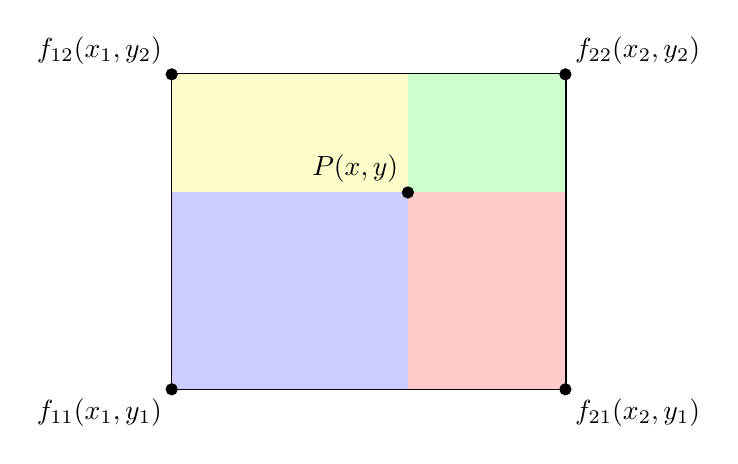
\begin{tikzpicture}
        % Define the rectangle vertices
        \coordinate (A) at (0,0);
        \coordinate (B) at (5,0);
        \coordinate (C) at (5,4);
        \coordinate (D) at (0,4);
        \coordinate (P) at (3,2.5); % Point d'interpolation
        
        % Draw rectangle
        \draw[thick] (A) -- (B) -- (C) -- (D) -- cycle;
        
        % Draw the perpendicular lines from P to the sides of the rectangle
        \draw[dashed] (P) -- (3,0);   % Vertical to the bottom side
        \draw[dashed] (P) -- (3,4);   % Vertical to the top side
        \draw[dashed] (P) -- (0,2.5); % Horizontal to the left side
        \draw[dashed] (P) -- (5,2.5); % Horizontal to the right side
        
        % Fill the areas
        \fill[blue!20]  (A) -- (3,0) -- (P) -- (0,2.5) -- cycle;
        \fill[red!20]   (B) -- (5,2.5) -- (P) -- (3,0) -- cycle;
        \fill[green!20] (C) -- (5,2.5) -- (P) -- (3,4) -- cycle;
        \fill[yellow!20] (D) -- (0,2.5) -- (P) -- (3,4) -- cycle;
        
        % Draw points
        \filldraw[black] (A) circle (2pt) node[anchor=north east] {$f_{11} (x_1, y_1)$};
        \filldraw[black] (B) circle (2pt) node[anchor=north west] {$f_{21} (x_2, y_1)$};
        \filldraw[black] (C) circle (2pt) node[anchor=south west] {$f_{22} (x_2, y_2)$};
        \filldraw[black] (D) circle (2pt) node[anchor=south east] {$f_{12} (x_1, y_2)$};
        \filldraw[black] (P) circle (2pt) node[anchor=south east] {$P (x, y)$};
        
        % Title
        %\node at (2.5,-1) {Interpolation Bilinéaire};
        %Interpolation Bilinéaire
    \end{tikzpicture}
    \caption{Schéma d'interpolation bilinéaire}
    %\label{fig:interpolation_IDW_rayon}
\end{figure}


\begin{comment}
    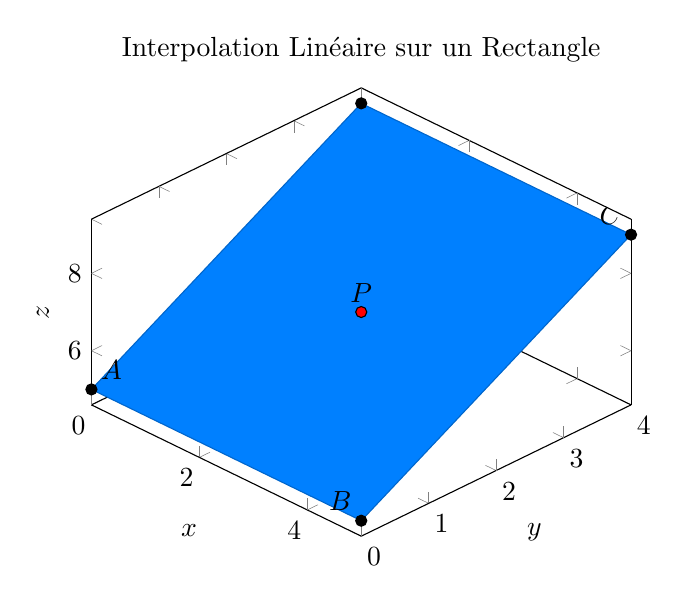
\begin{tikzpicture}
    \begin{axis}[
        view={45}{45},
        xlabel={$x$},
        ylabel={$y$},
        zlabel={$z$},
        colormap/cool,
        title={Interpolation Linéaire sur un Rectangle},
        ]

        % Define the vertices of the rectangle
        \addplot3[surf, mesh/rows=2, domain=0:5, domain y=0:4] 
            coordinates {(0,0,5) (5,0,5) (0,4,9) (5,4,9)};

        % Draw points for vertices and their labels
        \addplot3[only marks, mark=*] coordinates {(0,0,5) (5,0,5) (5,4,9) (0,4,9)};
        \addplot3[only marks, mark=*, mark options={fill=red}] coordinates {(2.5,2,7)};

        % Labels for the vertices and interpolated point
        \node at (axis cs:0,0,5) [anchor=south west] {$A$};
        \node at (axis cs:5,0,5) [anchor=south east] {$B$};
        \node at (axis cs:5,4,9) [anchor=south east] {$C$};
        \node at (axis cs:0,4,9) [anchor=south west] {$D$};
        \node at (axis cs:2.5,2,7) [anchor=south] {$P$};

    \end{axis}
    \end{tikzpicture}
\end{comment}


\subparagraph{Quadrilatère}

Regardons maintenant la dernière forme 2D rencontrée dans les solutions traitées par Antares : les quadrilatères.
Pour cela je n'ai pas trouvé de méthode satisfaisante dans la littérature.\cite{perronnet1998} Après plusieurs essais sur papier, je me suis concentré sur le fait que la méthode devait être continue, ce qui implique notamment que la valeur du point à interpoler doit tendre vers la valeur d'un sommet lorsque sa distance à ce dernier tend vers 0.
Une première vérification de la linéarité est aussi de vérifier qu'un point au milieu d'une forme 2D a comme valeur la moyenne de ses sommets.
Via cette démarche, j'ai imaginé, graphiquement, tracer des traits entre le point à interpoler et les sommets de la forme dans laquelle il se situe (tel que pour l'interpolation Barycentrique).
Cela permet de ne créer que 4 sous formes.
Ensuite pour déterminer le poids associé au sommet \( s_1 \), il faut multiplier entre elles les deux surfaces qui lui sont opposées, et bien entendu, le pondérer une fois les autres poids calculés.
Par opposées j'entends que ces surfaces ne sont composées d'aucune arrête ayant pour l'une de leurs extrémités le point d'interpolation. Ceci est important pour le 3D. Pour l'instant, je n'ai démontré que par l'expérimentation que cette méthode était linéaire.
Un point qui me perturbait était de faire des multiplications de surfaces, donc ordre 4, dans une méthode linéaire.
Mais contrairement à son nom, l'interpolation bilinéaire est en réalité quadratique avec un résultat linéaire.
On pourrait imaginer que, par chance, cette méthode soit quadratique.
Premièrement j'ai vérifié et ce n'est apparemment pas le cas.
Deuxièmement je pense que le quadratique n'englobe pas le linéaire dans le cas où nous nous basons uniquement sur les quatre points d'un quadrilatère.
% Effectivement, en 1D, si nous avons \(f(x_i)\) = 0 et \(f(x_{i+1})\) = 1, le résultat d'une variable linéaire serait 0,5 et celui d'une variable quadratique 0,25, si nous avons uniquement connaissance de ces deux points.
Normalement il faudrait s'appuyer sur plus de points pour le quadratique. 
Finalement, la demonstration pourrais se construire en montrant la linéarité selon les axes x et y indépendamment (comme pour le bilinéaire). En effet, sur la figure \ref{fig:quad} ci-dessous, nous remarquons que lors d'un déplacement selon l'horizontal, vers la droite, les surfaces \(\alpha\) et \(\gamma\) ne varient pas tandis que la surface \(\delta\) augment linéairement et \(\beta\) diminue linéairement aussi.
Voici l'équation :

\begin{equation}
    f(P) = \frac{f_{A} \cdot (\beta \times \gamma) + f_{B} \cdot (\gamma \times \delta) + f_{C} \cdot (\delta \times \alpha) + f_{D} \cdot (\alpha \times \beta)}{(\beta \times \gamma) + (\gamma \times \delta) + (\delta \times \alpha) + (\alpha \times \beta)}
\end{equation}
    

\begin{figure}[ht!]
    \centering
    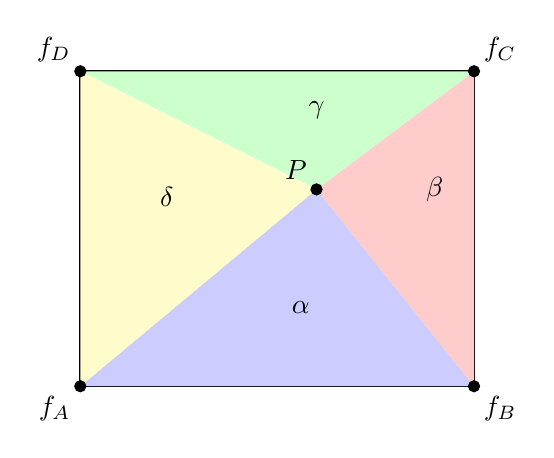
\begin{tikzpicture}
        % Define the rectangle vertices
        \coordinate (A) at (0,0);
        \coordinate (B) at (5,0);
        \coordinate (C) at (5,4);
        \coordinate (D) at (0,4);
        \coordinate (P) at (3,2.5); % Point d'interpolation
    
        % Draw rectangle
        \draw[thick] (A) -- (B) -- (C) -- (D) -- cycle;
    
        % Draw the interpolation lines parallel to the sides
        \draw[dashed] (P) -- (0,2.5); % Horizontal to the left side
        \draw[dashed] (P) -- (3,0);   % Vertical to the bottom side
        \draw[dashed] (P) -- (5,2.5); % Horizontal to the right side
        \draw[dashed] (P) -- (3,4);   % Vertical to the top side
    
        % Fill the areas
        \fill[blue!20]  (A) -- (P) -- (B) -- cycle;
        \fill[red!20]   (B) -- (P) -- (C) -- cycle;
        \fill[green!20] (C) -- (P) -- (D) -- cycle;
        \fill[yellow!20] (D) -- (P) -- (A) -- cycle;
    
        % Draw points
        \filldraw[black] (A) circle (2pt) node[anchor=north east] {$f_A$};
        \filldraw[black] (B) circle (2pt) node[anchor=north west] {$f_B$};
        \filldraw[black] (C) circle (2pt) node[anchor=south west] {$f_C$};
        \filldraw[black] (D) circle (2pt) node[anchor=south east] {$f_D$};
        \filldraw[black] (P) circle (2pt) node[anchor=south east] {$P$};
    
        % Add labels for the distances
        \node at (2.8, 1.0) {$\alpha$};%{$x_2 - x$};
        \node at (4.5, 2.5) {$\beta$};%{$y_2 - y$};
        \node at (3.0, 3.5) {$\gamma$};%{$x - x_1$};
        \node at (1.1, 2.4) {$\delta$};%{$y - y_1$};
    
        % Title
        %\node at (2.5,-1) {Interpolation dans un quadrilatère quelconque};
    
    \end{tikzpicture}
    \caption{Schéma d'interpolation dans un quadrilatère quelconque}
    \label{fig:quad}
    %\label{fig:interpolation_IDW_rayon}
\end{figure}

\vspace{0.5cm}  % OU \\[0pt plus 1fill] OU \newline OU flushleft, flushright, center


\paragraph{3D}
\subparagraph{Pavé droit : Trilinéaire}

Pour le 3D, si le maillage est structuré, alors la forme est le pavé droit. À ce moment, nous sommes dans le cas de l'interpolation dite trilinéaire. Encore une fois la formule se trouve facilement. Nous associons comme poids à un des huit sommets \( s_1 \) le volume opposé, construit de la sorte :

\begin{figure}[ht!]
    \centering
    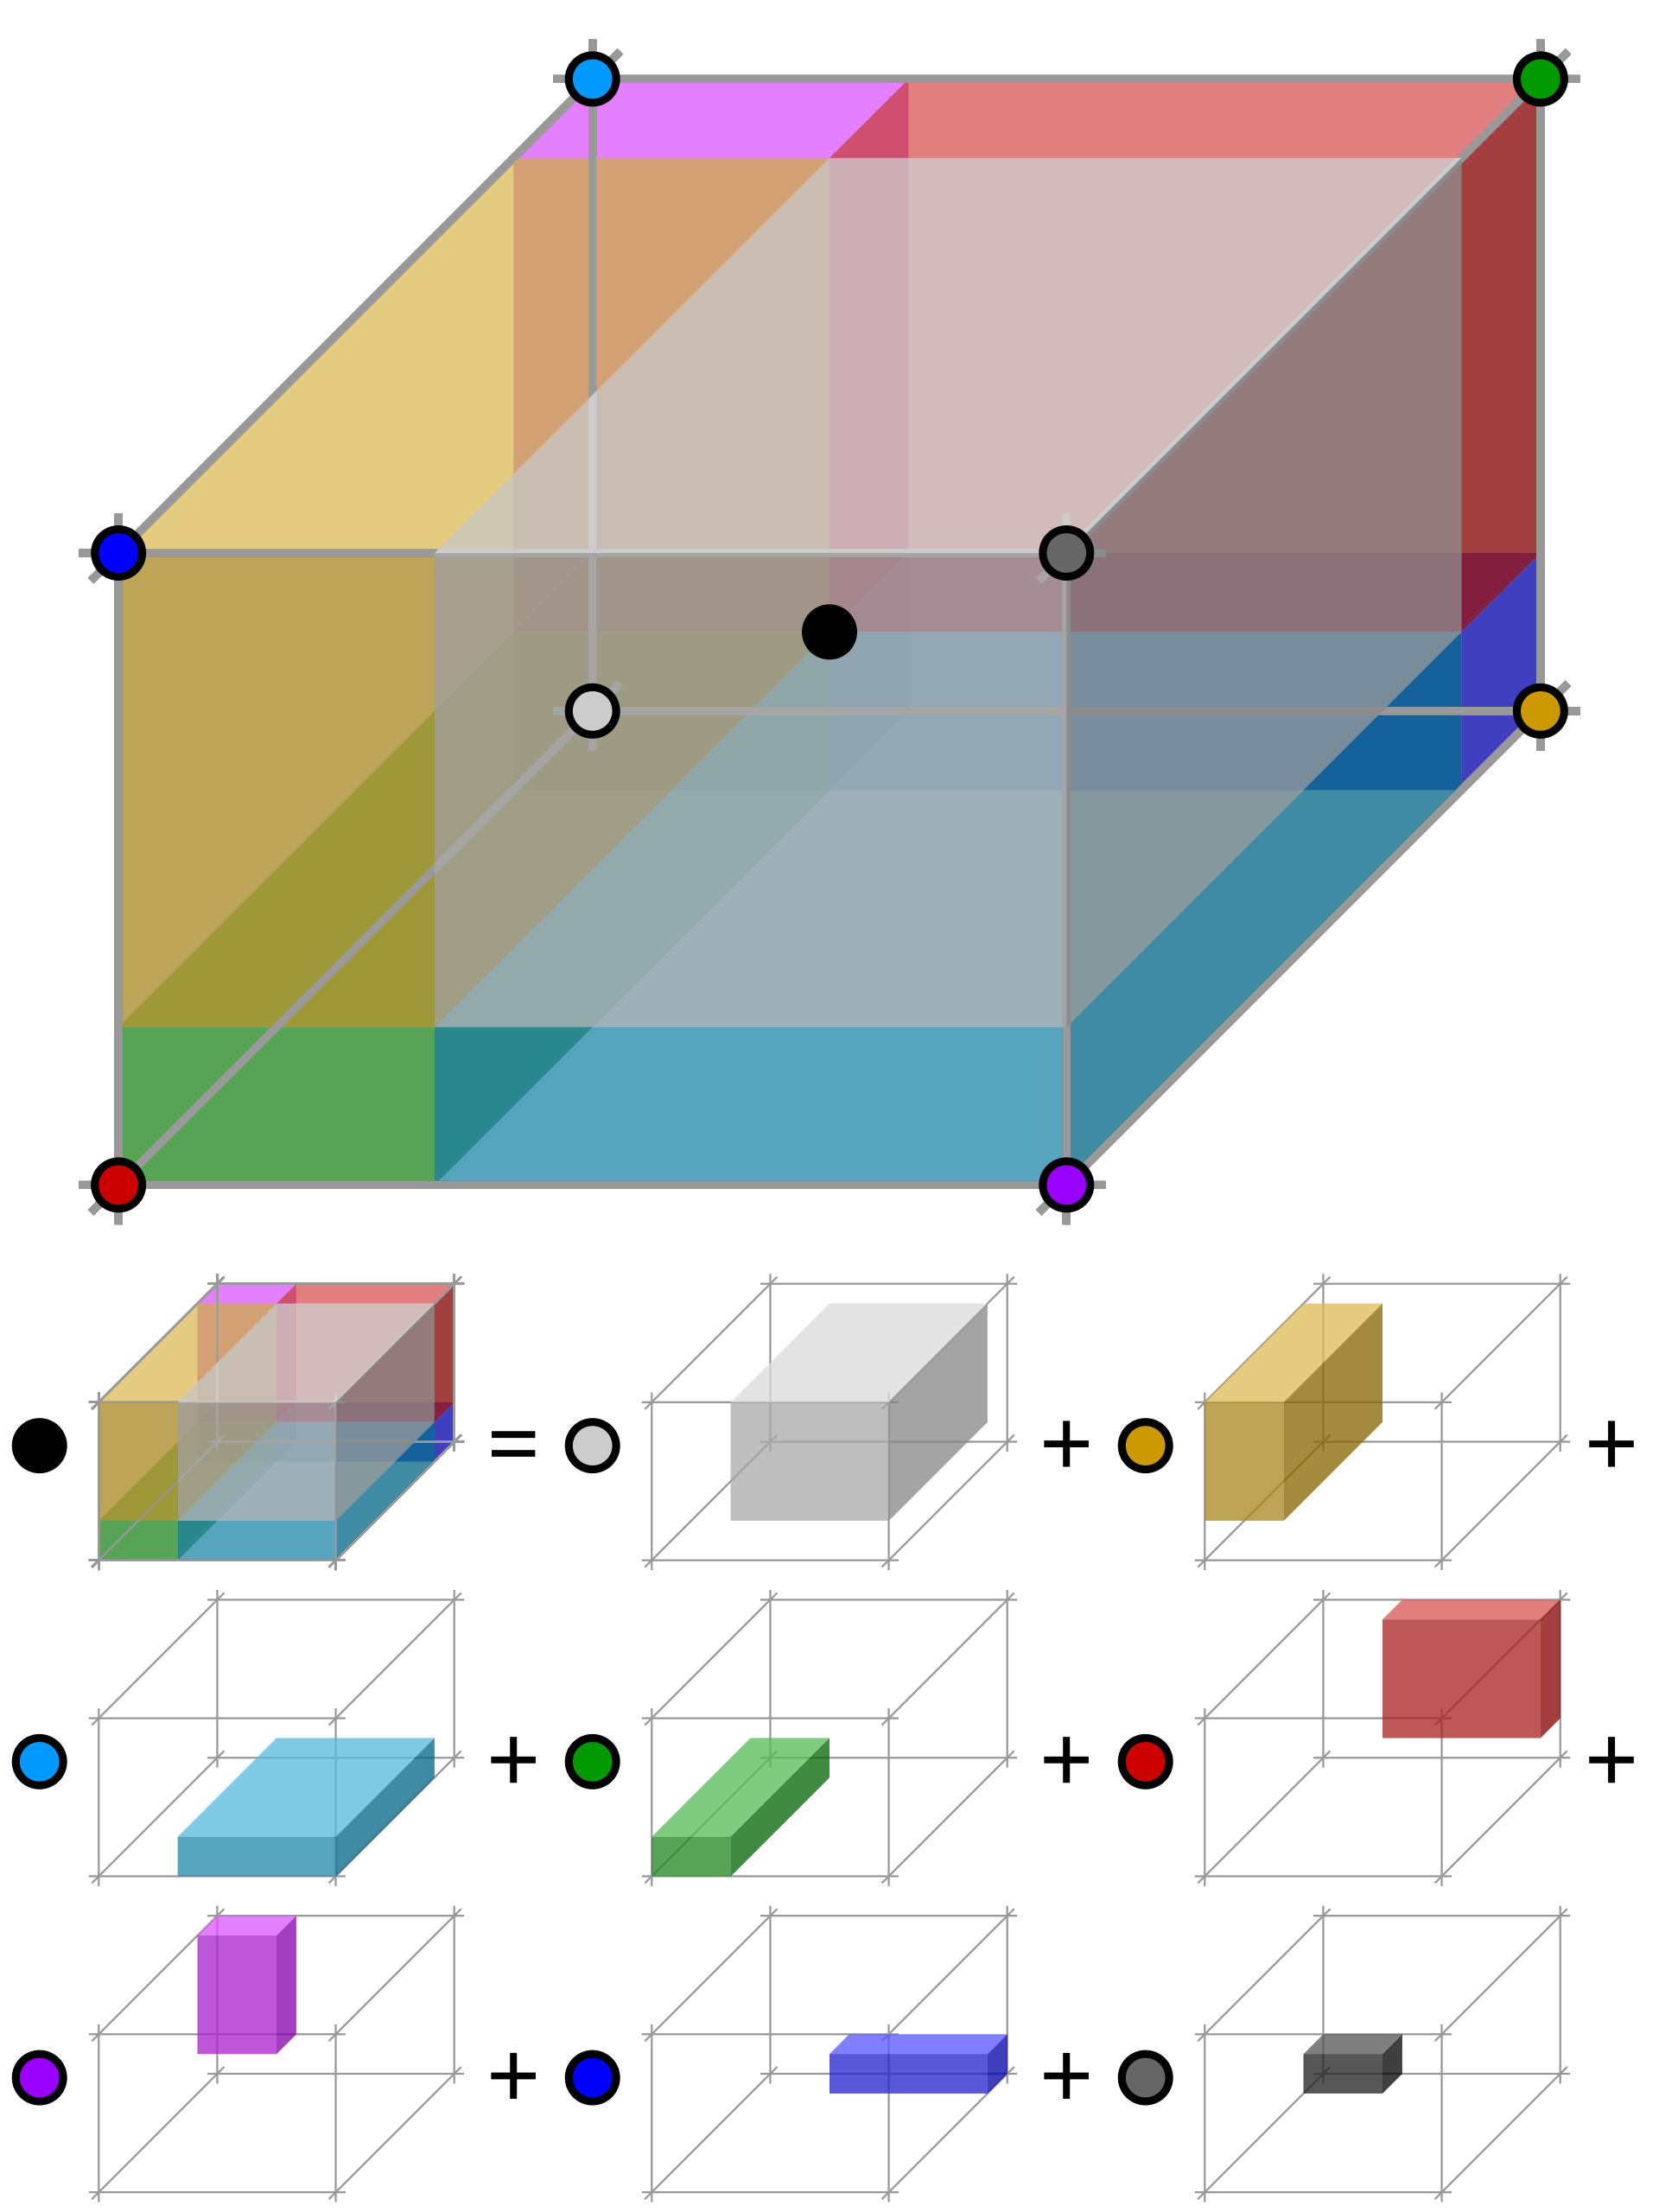
\includegraphics[width=0.4\textwidth]{images/Trilinear_interpolation_visualisation.svg.png}
    \caption{Schéma d'interpolation trilinéaire (source : Wikipédia)} %\footnote{Source:https://en.wikipedia.org/wiki/Trilinear_interpolation#/media/File:Trilinear_interpolation_visualisation.svg}}
    %\label{fig:https://en.wikipedia.org/wiki/Trilinear_interpolation#/media/File:Trilinear_interpolation_visualisation.svg}
\end{figure}

L'équation qui en découle est la suivante :

\begin{equation}
    f(x, y, z) = \sum_{i=0}^{1} \sum_{j=0}^{1} \sum_{k=0}^{1} f_{ijk} (1 - |x - x_i|)(1 - |y - y_j|)(1 - |z - z_k|)
\end{equation}

% Expliquer mathématiquement ? Ou plus tard dans le code ?  (quadrilatère non croisé, concave et convexes)

% En CFD il y a toujours des formes, même si c'est structuré, on peut unstructure.

\subparagraph{Thetraedre : Barycentrique étendu}

Pour le tétraèdre (une pyramide à base triangulaire quelconque), nous trouvons bien un volume opposé à chaque sommet. Opposé dans le sens où le sommet ne partage pas de segment avec le volume. Nous pouvons alors appliquer la même formule que pour le triangle, avec 4 volumes à la place de 3 surfaces.

\subparagraph{Prisme et pyramide et Hexaèdre}

Pour le prisme, la pyramide (à base quadrilatérale) et l’hexaèdre, une extension de la formule du quadrilatère sera faite.


La méthode ne fonctionne possiblement pas pour des prismes constitués de triangles non parallèles entre eux dans l'espace et/ou de surface différentes.


Note pour l'ordre supérieur : faire une transformation des formes qui aurait pu être utilisée en linéaire comme pour le cas du quadrilatère. \cite{camarero2024}



\subsection{Résumé des similitudes et différences des différentes méthodes}



\section{Implémentation de la méthode linéaire}

\subsection{La structure générale du code TreatmentInterpolation}


Le traitement d'interpolation d'Antares ne traite que des maillages ayant des valeurs uniquement au niveau des nœuds des cellules (pas entre).



EXPLICATION PLUS DÉTAILLER DU KDTREE

Après avoir recensé les différentes méthodes qui seraient applicables, ma seconde mission a été d'implémenter une interpolation linéaire dans Antares. Grâce à Nitrox, j'ai accès au code source de la librairie que je peux modifier. Le code 'interpolation.py' faisait environ 500 lignes. Il est orienté objet. Il prend comme arguments obligatoires la base source et la base cible et renvoie dans le cas le plus simple la base cible avec les valeurs interpolées.
De manière simplifiée, dans le code, les zones de la base source sont fusionnées puis nous parcourons les instants. 
Cette fusion permet de faire un KDTree (pour arbre à k-dimensions), qui permet concrètement de rechercher de manière efficace quels sont les \( N \) points de la base source les plus proches des points de la base cible (et les distances associées, utilisées dans la méthode 'idw').

Ensuite nous calculons l'interpolation via une des deux méthode 'principale' qui peut elle-même appeler d'autres fonctions ou méthodes d'Antares. % (\lstinline{__idw_interpolate_instant} ou \lstinline{__barycentrique_interpolate_instant})


///////// Les arguments de la méthode ajoutés et listage de ceux existants //////////// \label{arguments}


\subsection{Le Pseudo-algorithme}



Voici le pseudo-algorithme simplifié donnant l'architecture de la fonction linéaire du traitement interpolation.

\vspace{0.5cm}

\textbf{Initialisation :}

$\bullet$ Créer le KD-tree

$\bullet$ Créer une liste de listes \texttt{node\_to\_elements} qui permet de récupérer l'indice des éléments constitués par un certain point.

$\bullet$ Définir les points à interpoler

\vspace{0.5cm}

\textbf{Parcours des points à interpoler :}
\begin{list}{$\circ$}{\leftmargin=0.5cm \labelwidth=1cm \itemsep=0cm}
    \item Pour chaque point :
    \begin{list}{$\diamond$}{\leftmargin=0.5cm \labelwidth=1cm \itemsep=0cm}
        \item Si la distance au point le plus proche est inférieure à \texttt{tolerance} :
        \begin{list}{$\bullet$}{\leftmargin=0.5cm\labelwidth=1cm \itemsep=0cm}
            \item Le poids associé au \texttt{point cible} prend la valeur 1
            \item Le sommet associé au \texttt{point cible} prend la valeur du \texttt{point source} le plus proche
        \end{list}
        \item Sinon :
        \begin{list}{$\bullet$}{\leftmargin=0.5cm \labelwidth=1cm \itemsep=0cm}
            \item Récupérer les indices des éléments des points les plus proches\\
            $\circ$ Pour chaque élément pertinent :
            \begin{list}{$\bullet$}{\leftmargin=0.5cm\labelwidth=1cm \itemsep=0cm}
                \item Récupérer les coordonnées des sommets (points) de l'élément\\
                $\diamond$ Si le point est à l'intérieur de la forme de l'élément :
                \begin{list}{$\bullet$}{\leftmargin=0.5cm \labelwidth=1cm \itemsep=0cm}
                    \item Calculer les poids 'barycentriques'
                    \item Récupérer les indices des sommets (points) de la base source
                \end{list}
            \end{list}
        \end{list}
    \end{list}
    $\diamond$ Si le point n'est dans aucune cellule proche :
    \begin{list}{$\bullet$}{\leftmargin=0.5cm \labelwidth=1cm \itemsep=0cm}
        \item Le poids associé prend la valeur \texttt{numpy.nan} (cette valeur sera changée avant la mise à jour d'octobre)
    \end{list}
\end{list}

\vspace{0.5cm}

\begin{comment}
    Premièrement, dans \lstinline{__barycentrique_interpolate_instant}, nous récupérons le nombre de points maximal sur lequel nous allons nous appuyer pour l'interpolation, soit le nombre maximal de sommet des formes présentes dans le maillage.
    Nous récupérons les distances et indices du KDTree.
    Ensuite nous devons réarranger des indices qui se sont fait déplacer lors de la fusion des zones.
    Nous récupérons aussi différentes variables, comme les coordonnées des points, \dots
\end{comment}

%Nous récupérons d'une fonction définie plus bas (\lstinline{get_list_cell_type}) :
%(\lstinline{list_cell_type, max_node_index})

\noindent Dans le cas où le maillage est le même entre tous les instants, ou que l'utilisateur a déjà récupéré les poids (et autres valeurs utiles) nous ne recalculons pas tous les paramètres, ce qui permet une diminution significative du temps de calcul.

\vspace{0.5cm}

\textbf{Mise à jour de la base cible :}
\begin{list}{$\circ$}{\leftmargin=0.5cm \labelwidth=1cm \itemsep=0cm}
    \item Pour chaque variable à interpoler :
    \begin{list}{$\bullet$}{\leftmargin=0.5cm \labelwidth=1cm \itemsep=0cm}
        \item La variable de chaque nouveau point prend la valeur des poids calculés multiplié par la variable aux sommets (points) respectifs de la base source
    \end{list}
\end{list}


%Expliquer 'is point on cell', etc...

%% \subsection{Les difficultés}

\subsection{Optimisation du temps de calcul}

Plusieurs axes ont été exploités afin de diminuer le temps de calcul du traitement d'interpolation.

Le premier a été énoncé dans le pseudo-algorithme section précédente. Il s'agit de ne calculer qu'une seule fois le couple (poids, indices des points source) et autres paramètres puis de les enregistrer. Cela est utile dans deux cas :

- Entre les instants si la structure des deux bases restent inchangées.
C'est par exemple dans le cas des bases issues de solutions aéroacoustique. Dans mon cas test, la solution contient 200 instants, le temps de calcul est alors presque divisé par 200.

Dans le code, un test est fait pour savoir si tous les instants sont partagés (voir \ref{instants_partages}). Si oui, alors les poids et autres données nécessaires sont calculés (grace à la variable \texttt{computation}), mais pas le premier instant. Ensuite tous les instants seront calculés avec les données. Cela permet d'éviter d'enregistrer les coordonnées une seule fois et ainsi réduire le coût de mémoire.
Cet optimisation est faite automatiquement dans le traitement.

- Si le calcul sur la base source est réalisé plusieurs fois sans que sa structure ne soit changée, qu'elle ait un instant ou plusieurs instant partagée. /////////Attention, dans le cas où la structure du maillage est différent entre deux instants, cette dernière ne peut pas être utilisée///////////. Ceci arrive régulièrement, notamment lors de tests. Dans ce cas, il faut légèrement changer l'appel à la fonction, voici un exemple :

\begin{lstlisting}[caption=Exemple de réutilisation des données, label={lst:antares}]
    import antares
    from copy import deepcopy
    # deepcopy est utilise pour s'assurer que la 'target_base' ne soit pas calculee par le traitement

    myt = antares.Treatment('interpolation')
    myt['source'] = source_base
    myt['target'] = deepcopy(target_base)
    myt['get_data'] = True
    result1, data = myt.execute()

    # 'data' peut etre enregistre sur votre ordinateur par exemple, pour pouvoir etre appele plus tard

    myt = antares.Treatment('interpolation')
    myt['source'] = source_base
    myt['target'] = target_base
    myt['data'] = data
    result2 = myt.execute()
\end{lstlisting}

Ici, \texttt{result2} aura été calculé beaucoup plus rapidement que \texttt{result1}.

De plus ce changement est aussi appliqué à la méthode IDW sans poser de problème de rétrocompatibilité, car les résultats sont inchangés.

\vspace{0.5cm}

La méthode linéaire était initialement 200 à 500 fois plus lente que IDW. J'ai donc fait du 'profiling' pour savoir quelles lignes de code étaient les plus coûteuses. J'ai remplacé des listes par des arrays, ce qui augmente la rapidité d'accès aux éléments de ce denier en mémoire.
J'ai aussi optimisé le test de localisation d'un point dans une cellule et de calcul des poids.
Je calcule d'abord les surfaces créées par le point cible avec les sommets puis, je calcule le volume de la cellule. Si ces volumes sont égaux à une erreur numérique près, alors le point est dans la cellule et j'ai les poids. Sinon je sais qu'il faut chercher ailleurs.

\vspace{0.5cm}

Une autre idée a été testée pour réduire le temps de calcul. Elle reste linéaire, mais ne donne pas forcément le même résultat (lorsque la variable à interpoler est non-linaire, sinon le résultat reste la solution analytique). Cette idée est décrite uniquement pour le cas 2D par soucis de simplicité de visualisation, mais est similaire pour le 3D.

Le principe est de ne pas calculer tout ce qui touche à la connectivité, car c'est ce qui augmente significativement le temps de calcul.
Nous allons alors chercher les 3 points les plus proches (4 en 3D). En reliant les sommets, cela donnera une forme dite non croisée. 
Ensuite, nous faisons le calcul des barycentres et appliquons la même méthode qu'au-dessus.
La différence ici est que le point cible n'est pas forcément dans la forme décrite par les 3 points les plus proches.



\begin{figure}[H]
    \centering
    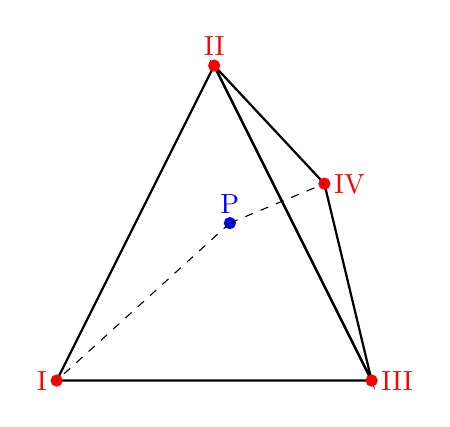
\begin{tikzpicture}
        \centering
        % Triangle initial
        \coordinate (I) at (0,0);
        \coordinate (II) at (2,4);
        \coordinate (III) at (4,0);
        \coordinate (P) at (2.2,2.0); % Point P (plus proche du nouveau triangle)

        % Nouveau triangle
        \coordinate (IV) at (3.4,2.5);

        % Draw the initial triangle
        \draw[thick] (I) -- (II) -- (III) -- cycle;

        % Draw the new triangle
        \draw[thick] (II) -- (III) -- (IV) -- cycle;

        % Draw point P
        \filldraw[blue] (P) circle (2pt) node[anchor=south] {P};

        % Label the vertices of the initial triangle
        \filldraw[red] (I) circle (2pt) node[anchor=east] {I};
        \filldraw[red] (II) circle (2pt) node[anchor=south] {II};
        \filldraw[red] (III) circle (2pt) node[anchor=west] {III};

        % Label the vertices of the new triangle
        \filldraw[red] (IV) circle (2pt) node[anchor=west] {IV};

        % Draw lines from P to vertices
        \draw[dashed] (P) -- (IV);
        \draw[dashed] (P) -- (I);

        % Title
        %\node at (4,-1) {P plus proche de IV que du sommet le plus éloigné du triangle dans lequel il se trouve};
    \end{tikzpicture}
    \caption{Schéma de sélection du deuxième point le plus proche}
    \label{fig:deux_pt}
%\label{fig:interpolation_IDW_rayon}
\end{figure}


Alors nous pourrions avoir une ou des surfaces formées par le point cible qui sortent du triangle initial (et la somme des surfaces ne serait pas égale à la surface du triangle initial). Mais pour respecter la linéarité, il suffit de faire le même calcul en prenant en compte le fait que la ou les deux surface(s) entièrement extérieures à la forme sont négatives. La figure ci-dessous est un zoom sur le schéma \ref{fig:deux_pt}.

\begin{figure}[H]
    \centering
    \begin{tikzpicture}
        % Triangle initial
        \coordinate (II) at (2*1.5,4*1.5);
        \coordinate (III) at (4*1.5,0);
        \coordinate (P) at (2.2*1.5,2.0*1.5); % Point P (plus proche du nouveau triangle))
        \coordinate (IV) at (3.4*1.5,2.5*1.5);
    
        % Draw point P
        \filldraw[blue] (P) circle (2pt) node[anchor=east] {P};
    
        % Label the vertices of the initial triangle
        \filldraw[red] (II) circle (2pt) node[anchor=south] {II};
        \filldraw[red] (III) circle (2pt) node[anchor=west] {III};
    
        % Label the vertices of the new triangle
        \filldraw[red] (IV) circle (2pt) node[anchor=west] {IV};
    
        % Colorer les surfaces, avec une surface négative
        \fill[blue!20] (II) -- (P) -- (IV) -- cycle;
        \fill[green!20, opacity=1.0] (III) -- (P) -- (IV) -- cycle;
        % Utilisation de hachures pour indiquer une surface négative
        \fill[pattern=north west lines, pattern color=red, opacity=0.7] (P) -- (III) -- (II) -- cycle;
    
        % Draw the 'outside' triangle
        \draw[thick] (II) -- (III) -- (IV) -- cycle;
    
        % Draw lines from P to vertices
        \draw[thick] (P) -- (IV);
        \draw[thick] (P) -- (II);
        \draw[thick] (P) -- (III);
    
        % Ajouter des annotations pour indiquer la surface négative
        %\node at (2.1*1.5,2.15*1.5) [anchor=west] {Surface};
        %\node at (2.1*1.5,2.15*1.5-0.4) [anchor=west] {négative};
        \node at (3, 1) [anchor=east] {
            \begin{tikzpicture}[baseline]
                \fill[pattern=north west lines, pattern color=red, opacity=0.7] (0,0) rectangle (0.5,0.2);
            \end{tikzpicture}
            \hspace{0.1cm} Surface négative
        };
        %\node at (3, 1) [anchor=east] {Surface négative};
        \draw[->, thick] (3, 1) -- (4.0, 2.9);

        %\node at (2.5*1.5, 1.5*1.5) [anchor=north] {\textbf{-}};
    \end{tikzpicture}    
    \caption{Illustration de la surface négative avec le point P}
    \label{fig:surface_negative}
\end{figure}


N'ayant pas trouvé une façon simple de savoir si la surface était négative, par manque de temps et crainte de l'ajout de complexité (ce qui augmente le temps de calcul), cette méthode n'a pas été implémentée.
Cela permet aussi une extrapolation linéaire sans créer d'erreur.




////// C'est clair ou il faudrait illustrer la surface 'rouge' autrement ? ////////

////// Comment avoir le nom de (conf ou article ou rapport ou livre, ...) depuis un DOI ou sur ResearchGate ? /////////

\begin{comment}
    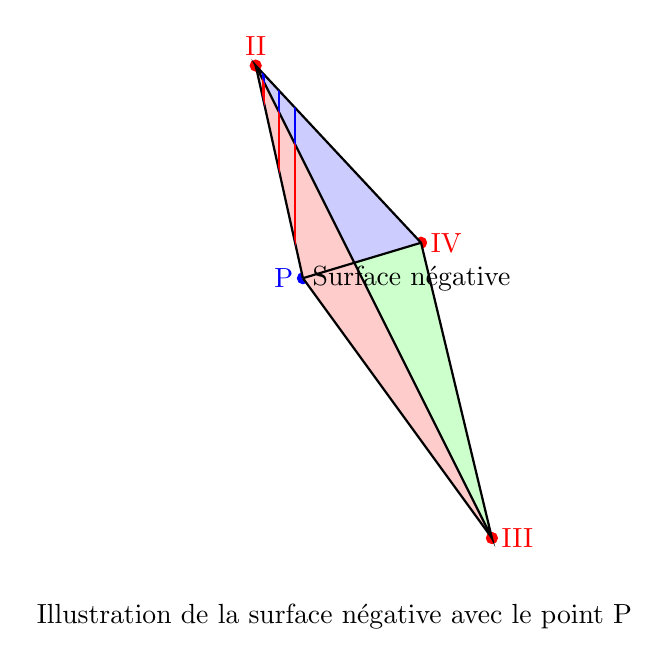
\begin{tikzpicture}
    \centering
    % Triangle initial
    \coordinate (II) at (2*1.5,4*1.5);
    \coordinate (III) at (4*1.5,0);
    \coordinate (P) at (2.4*1.5,2.2*1.5); % Point P (plus proche du nouveau triangle))
    \coordinate (IV) at (3.4*1.5,2.5*1.5);

    % Draw point P
    \filldraw[blue] (P) circle (2pt) node[anchor=east] {P};

    % Label the vertices of the initial triangle
    \filldraw[red] (II) circle (2pt) node[anchor=south] {II};
    \filldraw[red] (III) circle (2pt) node[anchor=west] {III};

    % Label the vertices of the new triangle
    \filldraw[red] (IV) circle (2pt) node[anchor=west] {IV};

    % Colorer les surfaces, avec une surface négative
    \fill[blue!20] (II) -- (P) -- (IV) -- cycle;
    \fill[green!20] (III) -- (P) -- (IV) -- cycle;
    \fill[red!20] (P) -- (III) -- (II) -- cycle; % Cette surface sera considérée comme négative

    % Draw the 'outside' triangle
    \draw[thick] (II) -- (III) -- (IV) -- cycle;

    % Draw lines from P to vertices
    \draw[thick] (P) -- (IV);
    \draw[thick] (P) -- (II);
    \draw[thick] (P) -- (III);

    % Hachures manuelles pour la surface bleue
    \begin{scope}
        \clip (II) -- (P) -- (IV) -- cycle;
        \foreach \x in {1.5,1.7,...,3.5} {
            \draw[blue, thick] (\x,-1) -- (\x,6);
        }
    \end{scope}

    % Hachures manuelles pour la surface verte
    \begin{scope}
        \clip (III) -- (P) -- (IV) -- cycle;
        \foreach \x in {1.5,1.7,...,3.5} {
            \draw[green, thick] (\x,-1) -- (\x,6);
        }
    \end{scope}

    % Hachures manuelles pour la surface rouge (négative)
    \begin{scope}
        \clip (P) -- (III) -- (II) -- cycle;
        \foreach \x in {1.5,1.7,...,3.5} {
            \draw[red, thick] (\x,-1) -- (\x,6);
        }
    \end{scope}

    % Ajouter des annotations pour indiquer la surface négative
    \node at (2.4*1.5,2.2*1.5) [anchor=west] {Surface négative};
    
    % Title
    \node at (4,-1) {Illustration de la surface négative avec le point P};
\end{tikzpicture}
\end{comment}

%\subsection{Le résultat}


\section{Tests}
% \section{Les différentes méthodes d'interpolation}
\subsection{Tests unitaires}
Des codes de tests ont été créés en même temps que l'implémentation de l'interpolation linéaire, pour tester si cette dernière fonctionne correctement sur des cas simples.
L'idée est de créer une base source avec une variable linéaire et une base cible avec des points décalés. Ensuite on teste l'interpolation retourne bien la valeur analytique espérée sur tous les types de cellules. Ce test est effectué très simplement avec une commande dans le terminal ou lors d'un git push vers Nitrox.



\subsection{Tests sur des cas industriels}

\begin{figure}[H]
    \centering
    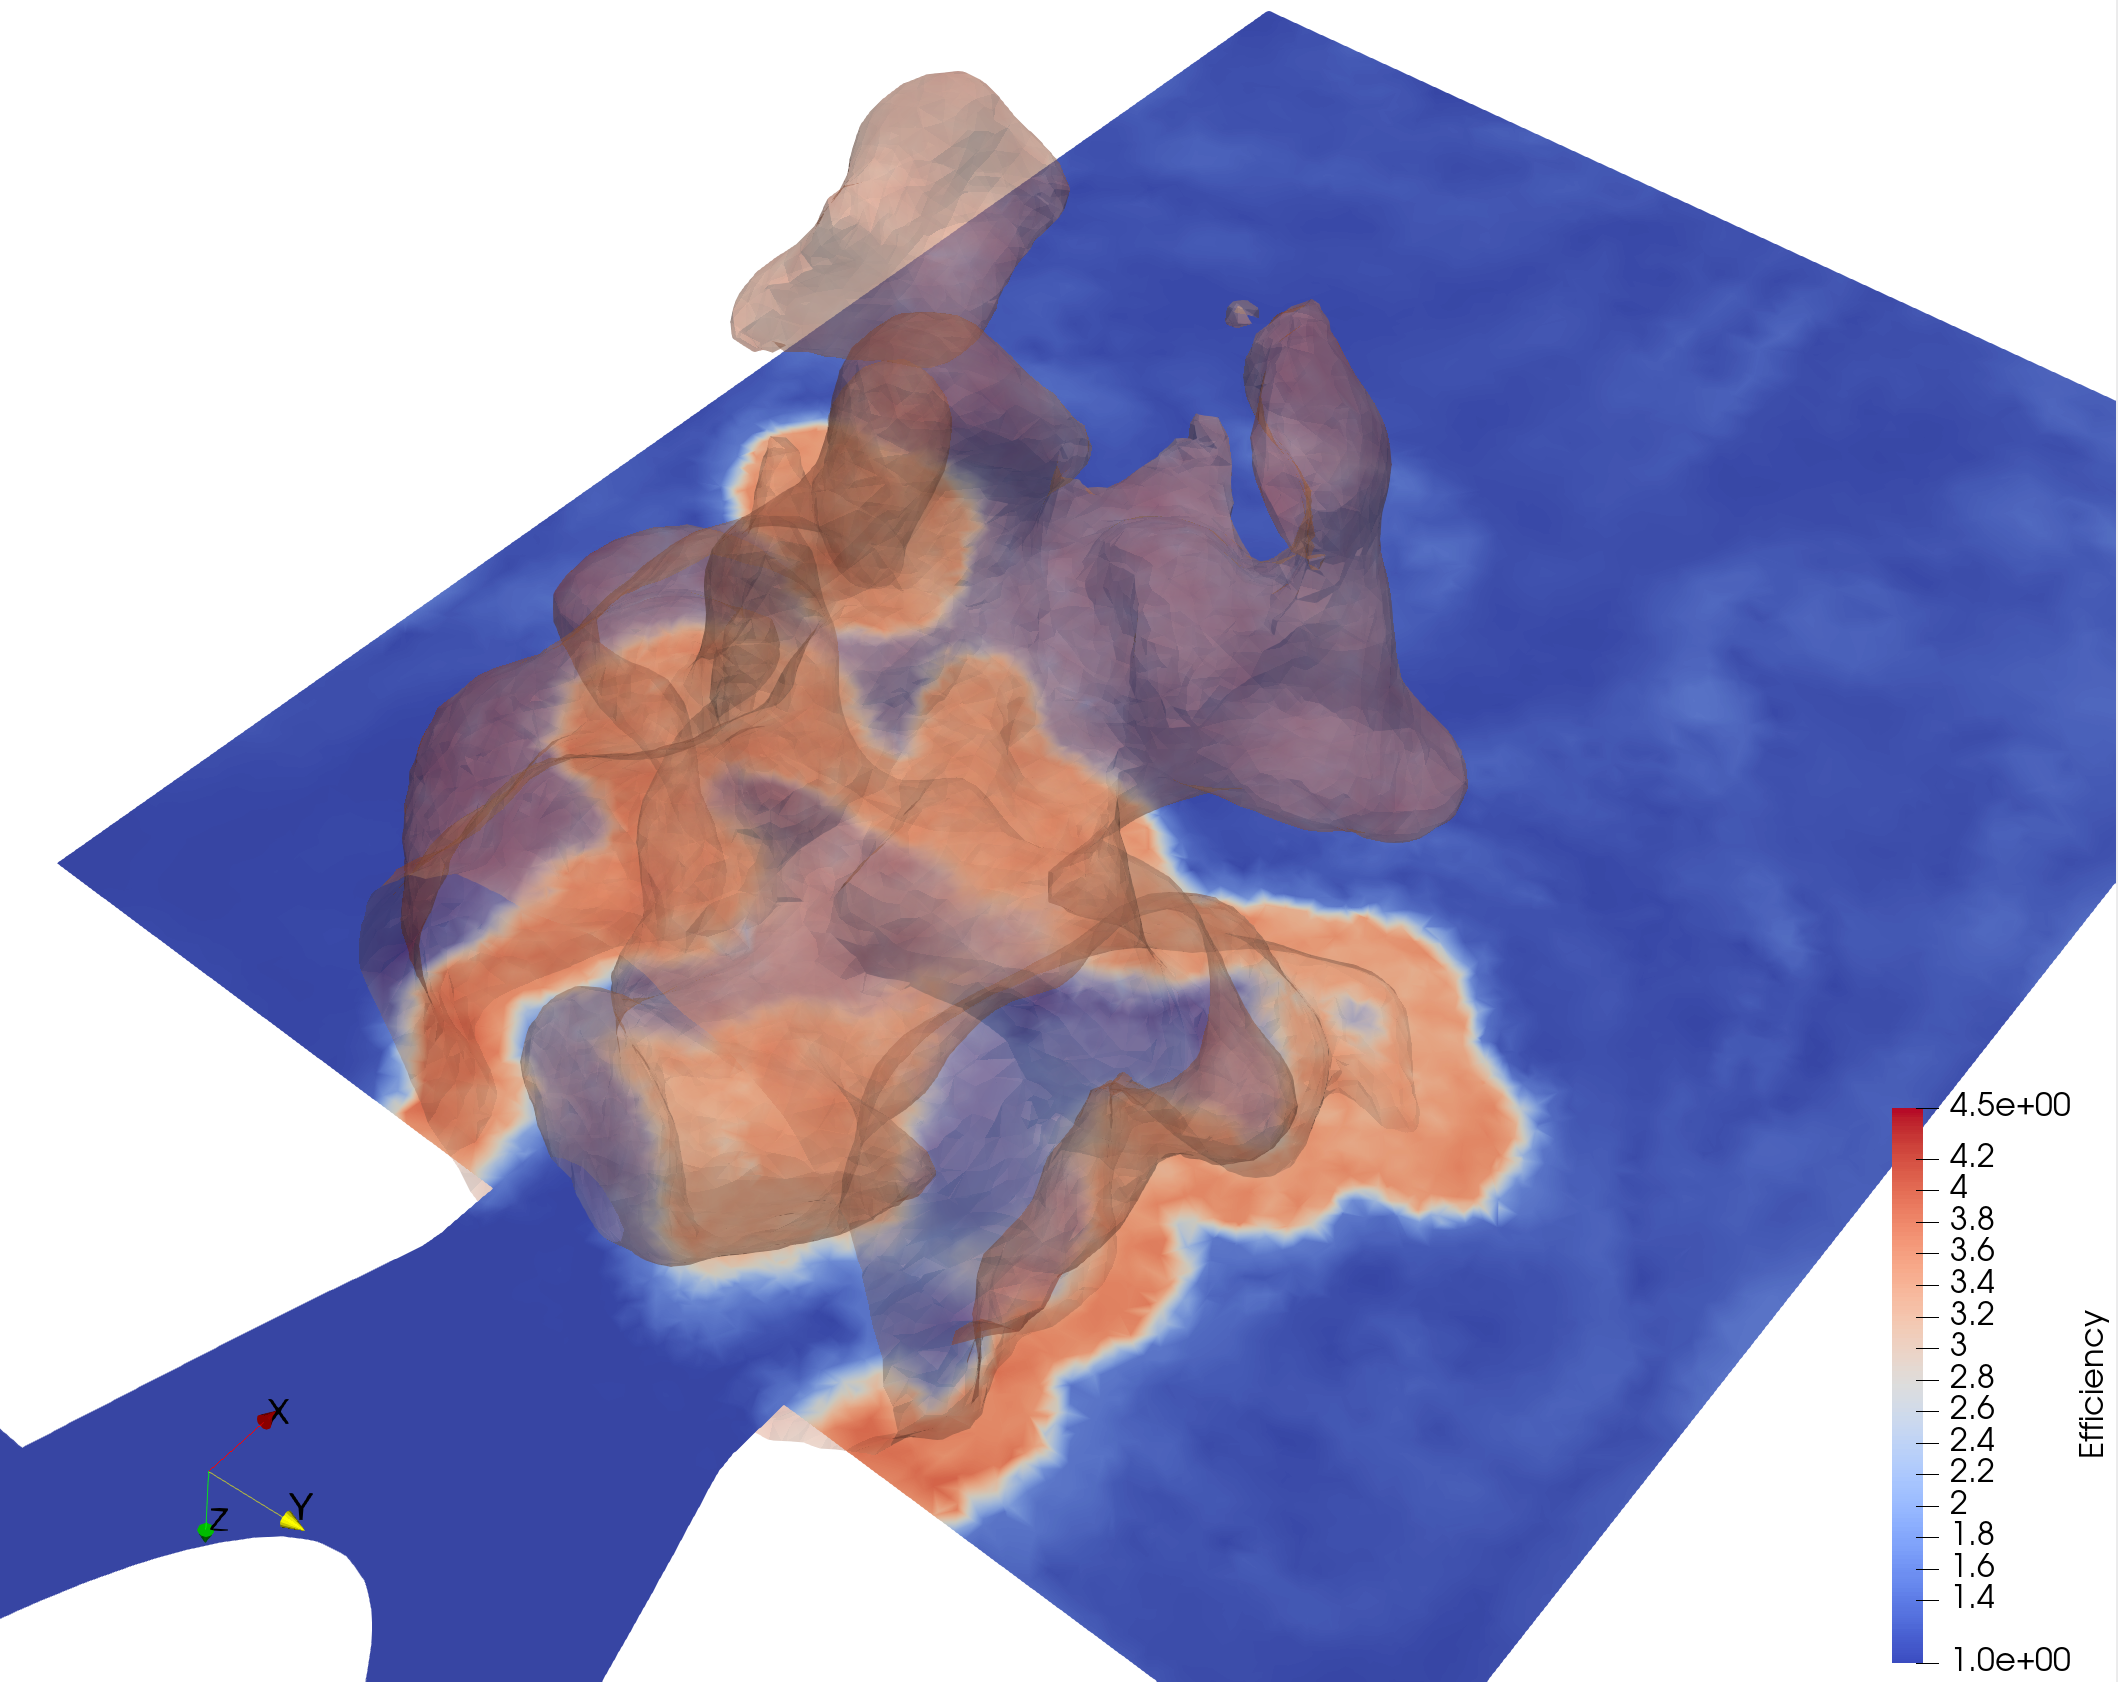
\includegraphics[width=0.50\textwidth]{images/cb-IDW.png}
    \caption{Interpolation IDW sur une coupe d'une chambre de combustion avec isosurface de la flame}
    \label{fig:cb-IDW}
\end{figure}

\begin{figure}[H]
    \centering
    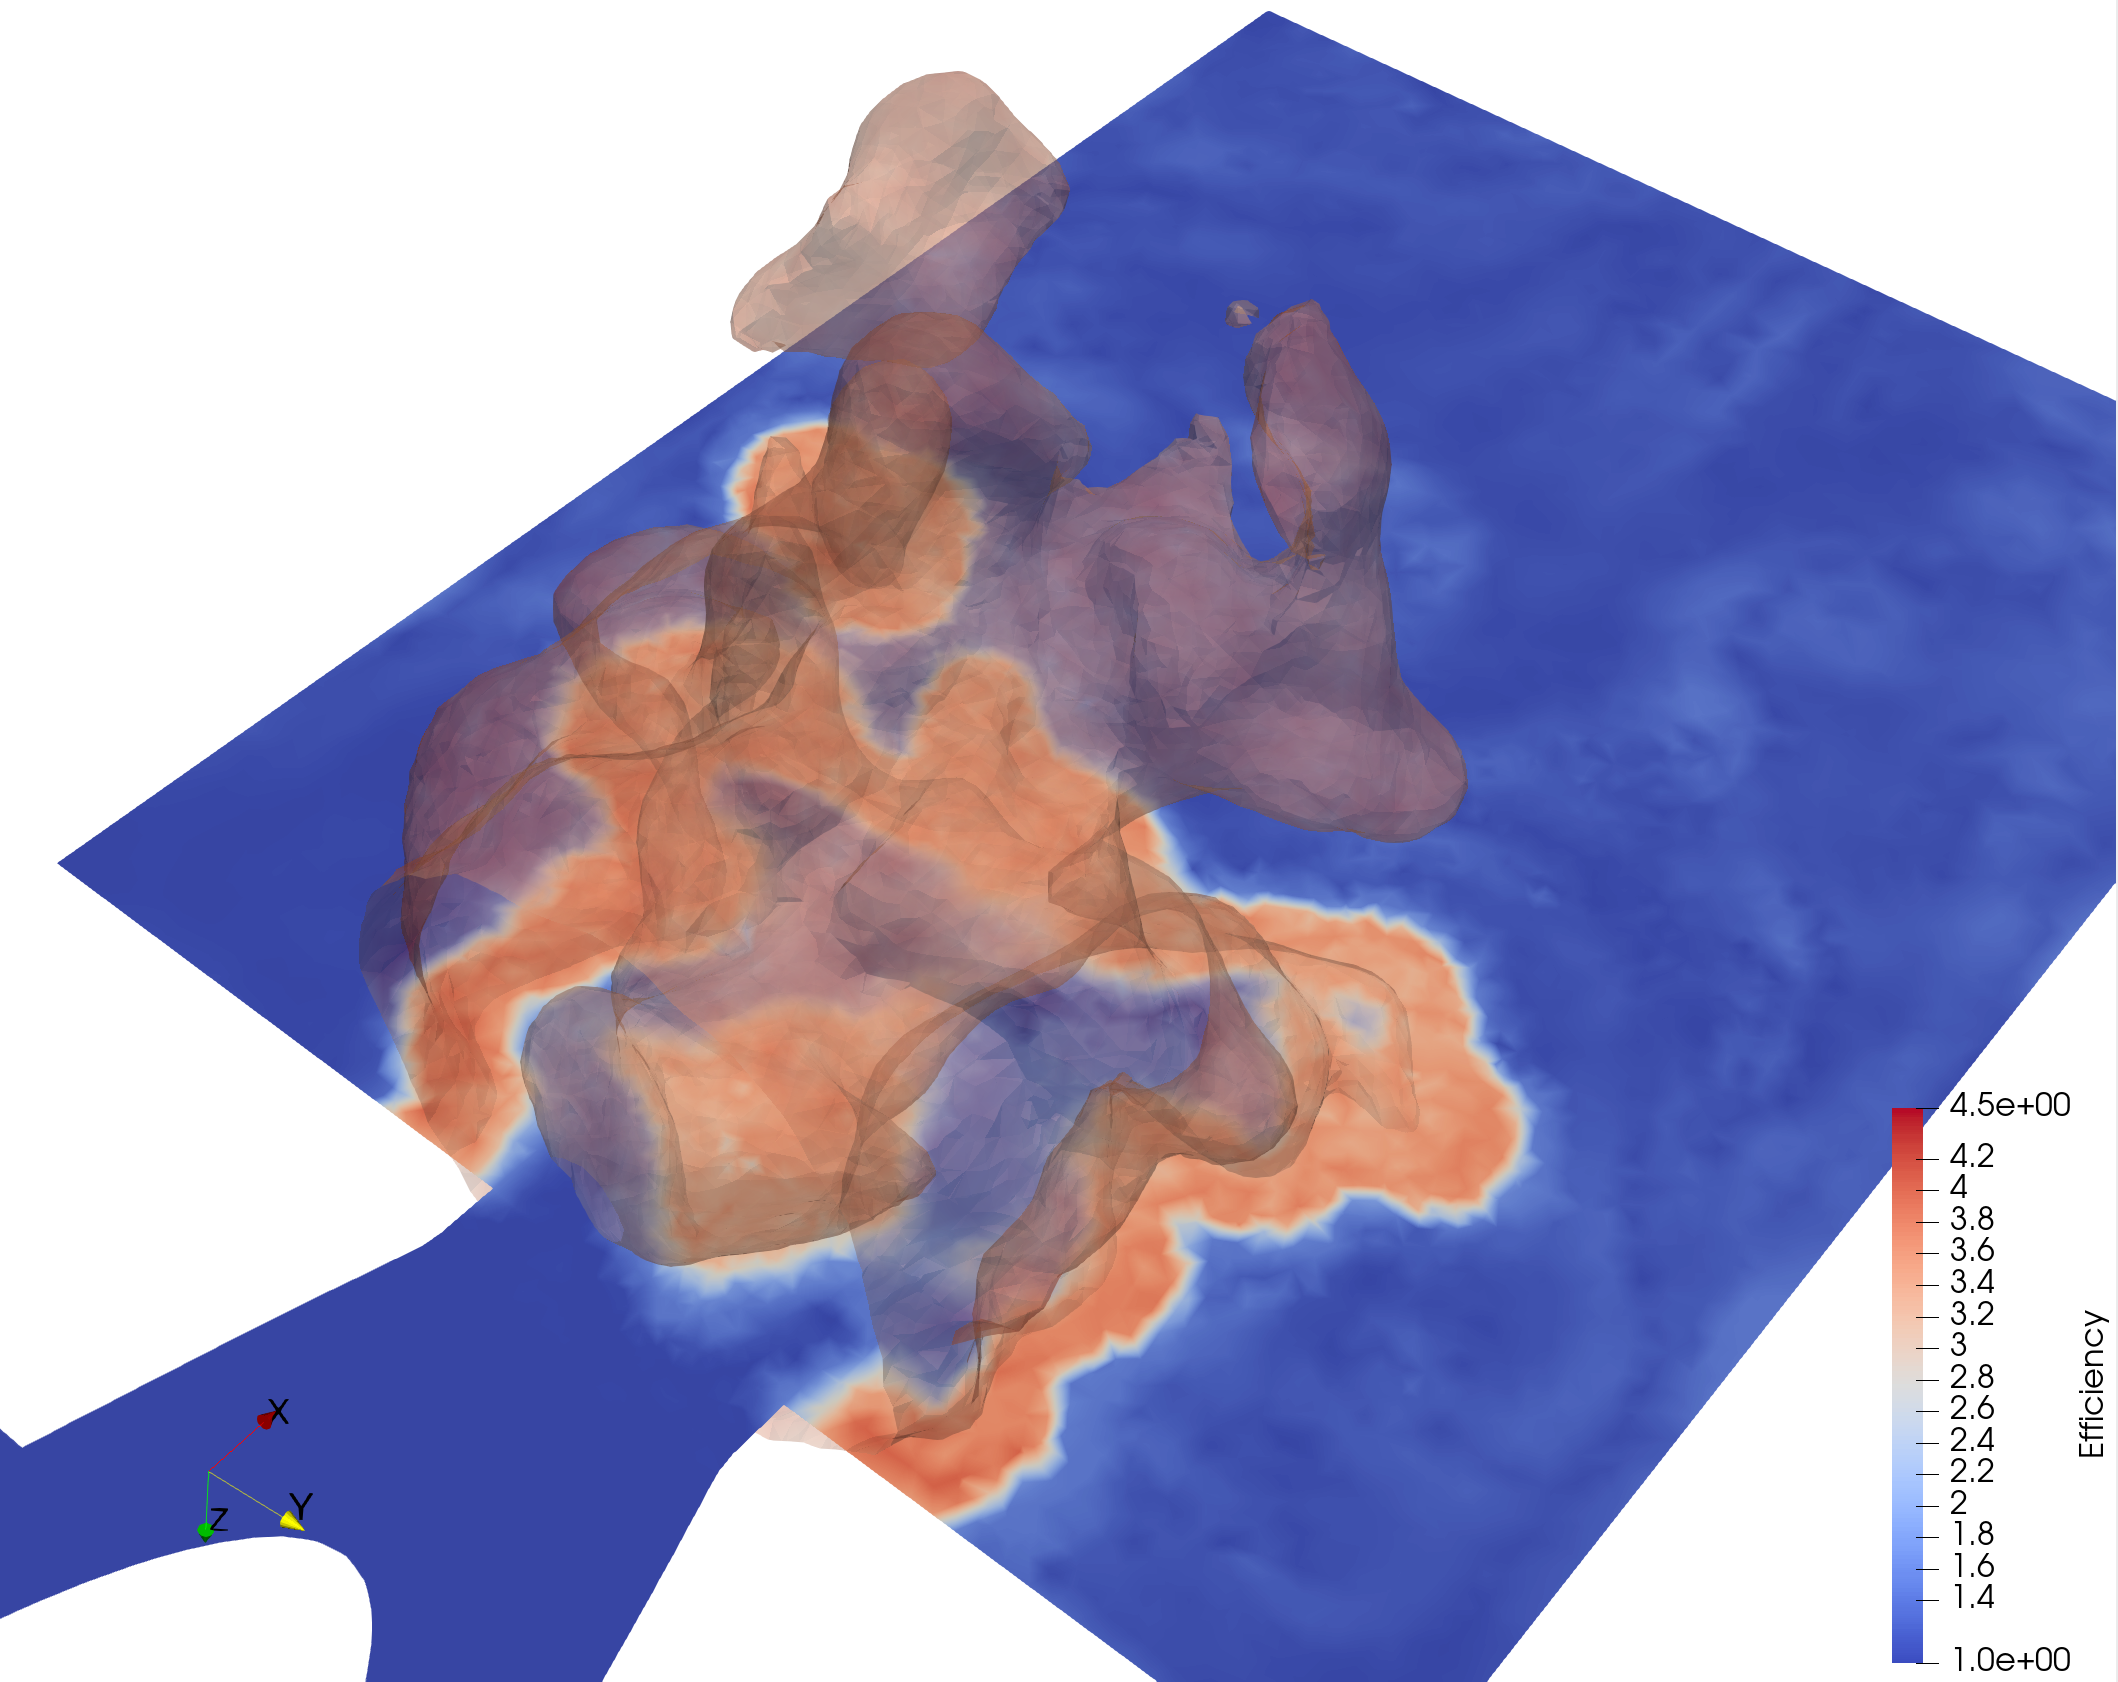
\includegraphics[width=0.50\textwidth]{images/cb-lineaire.png}
    \caption{Interpolation linéaire sur une coupe d'une chambre de combustion}
    \label{fig:cb-lineaire}
\end{figure}


Ensuite, des tests ont été réalisés sur des cas d'applications plus conséquents et complexes, comme l'intersection d'un plan cible dans le résultat d'une simulation de chambre de combustion. 




BIEN AFFICHER QUE LES Paramètres optimaux sont n-10 - p-10

À droit n=10, p=10. Rapports d'amplitude : idw : 101.88 %  Bary : 47.08 %. pour dipole et quadripôle

Carlos a développé l'outil permettant de déterminer le résultat acoustique, à grande distance, à partir d'une surface, en utilisant les équations de Ffowcs Williams – Hawkings. Le résultat acoustique sont les petites variations de pression, impliquant du son (à différentes fréquences et amplitudes). En pratique, pour les utilisateurs d'Antares, cette surface est définie dans un maillage 'solution' où nous avons le résultat de la pression en différents points et différents instants.

% Paramètres d'IDW
\subsection{Tests sur les paramètres de la méthode IDW}

\subsection{Tests sur des cas d'aéroacoustique}

\cite{schoder2019}

Une amélioration possible de l'interpolation pour le cas de l'aéroacoustique serait d'utiliser la méthode d'interpolation par partie décrite dans des articles de l’ONERA\cite{cunha2011}\cite{cunha2016}




... (\url{https://cerfacs.fr/antares/}) : 


\begin{itemize}
    \item TreeMesh 
    %Ici, le maillage DGMultiMesh dépend directement du solver DGMulti en fonction du type de géométrie utilisée, il faut donc le passer en argument.
\end{itemize}


